\documentclass[supercite]{Experimental_Report}

\title{~~~~~~计算机视觉实验三~~~~~~}
\author{崔昊阳}
\school{计算机科学与技术学院}
\classnum{CS2104}
\stunum{U202115415}
\instructor{刘康}
\date{2023年12月7日}

\usepackage{algorithm, multirow}
\usepackage{algpseudocode}
\usepackage{amsmath}
\usepackage{amsthm}
\usepackage{framed}
\usepackage{mathtools}
\usepackage{subcaption}
\usepackage{xltxtra}
\usepackage{bm}
\usepackage{tikz}
\usepackage{tikzscale}
\usepackage{pgfplots}
\usepackage{listings}
\lstset{
    backgroundcolor = \color{white},    % 背景色
    basicstyle = \small\ttfamily,           % 基本样式 + 小号字体
    rulesepcolor= \color{white},             % 代码块边框颜色
    breaklines = true,                  % 代码过长则换行
    numbers = left,                     % 行号在左侧显示
    numberstyle = \small,               % 行号字体
    keywordstyle = \color{blue}\bfseries,      % 关键字颜色
	identifierstyle=\color{purple}, 		% 标识符颜色
    commentstyle =\color{green},        % 注释颜色
    stringstyle = \color{green},          % 字符串颜色
    frame = None,                  % 用(带影子效果)方框框住代码块
    showspaces = false,                 % 不显示空格
    columns = flexible,                    % 字间距固定
}

\pgfplotsset{compat=1.16}

\newcommand{\cfig}[3]{
  \begin{figure}[H]
    \centering
    \includegraphics[width=#2\textwidth]{images/#1.tikz}
    \caption{#3}
    \label{fig:#1}
  \end{figure}
}

\newcommand{\sfig}[3]{
  \begin{subfigure}[b]{#2\textwidth}
    \includegraphics[width=\textwidth]{images/#1.tikz}
    \caption{#3}
    \label{fig:#1}
  \end{subfigure}
}

\newcommand{\xfig}[3]{
  \begin{figure}[H]
    \centering
    #3
    \caption{#2}
    \label{fig:#1}
  \end{figure}
}

\newcommand{\rfig}[1]{\autoref{fig:#1}}
\newcommand{\ralg}[1]{\autoref{alg:#1}}
\newcommand{\rthm}[1]{\autoref{thm:#1}}
\newcommand{\rlem}[1]{\autoref{lem:#1}}
\newcommand{\reqn}[1]{\autoref{eqn:#1}}
\newcommand{\rtbl}[1]{\autoref{tbl:#1}}

\algnewcommand\Null{\textsc{null }}
\algnewcommand\algorithmicinput{\textbf{Input:}}
\algnewcommand\Input{\item[\algorithmicinput]}
\algnewcommand\algorithmicoutput{\textbf{Output:}}
\algnewcommand\Output{\item[\algorithmicoutput]}
\algnewcommand\algorithmicbreak{\textbf{break}}
\algnewcommand\Break{\algorithmicbreak}
\algnewcommand\algorithmiccontinue{\textbf{continue}}
\algnewcommand\Continue{\algorithmiccontinue}
\algnewcommand{\LeftCom}[1]{\State $\triangleright$ #1}

\newtheorem{thm}{定理}[section]
\newtheorem{lem}{引理}[section]

\colorlet{shadecolor}{black!15}

\theoremstyle{definition}
\newtheorem{alg}{算法}[section]

\def\thmautorefname~#1\null{定理~#1~\null}
\def\lemautorefname~#1\null{引理~#1~\null}
\def\algautorefname~#1\null{算法~#1~\null}

\begin{document}

\maketitle

\clearpage

\pagenumbering{Roman}

\tableofcontents[level=2]

\clearpage

\pagenumbering{arabic}

\section{实验要求}
任务要求:设计一个卷积神经网络,输入为两张 MNIST 手写体数字图片,如果两张图片为同一个数字(注意,非同一张图片),输出为 1,否则为 0。

从 MNIST 数据集的训练集中选取 10\% 作为本实验的训练图片,从 MNIST 数据集的测试集中选取 10\% 作为本实验的测试图片。请将该部分图片经过适当处理形成一定数量的用于本次实验的训练集和测试集。

注意事项:
\begin{enumerate}
	\item 深度学习框架任选。
	\item 实验报告需包含训练集和测试集构成、神经网络架构、每一轮 mini-batch 训练后的模型在训练集和测试集上的损失、最终的训练集和测试集准确率,以及对应的实验分析。
	\item 将代码和实验报告打包成 ZIP 压缩包,以“姓名-学号-实验报告\#”命名,比如“张三-2020XXX-实验报告一.zip”,提交到学习通。
	\item 截止时间为 1 月 3 号下午 2:00。
\end{enumerate}

\section{数据处理}
\subsection{数据集的获取和处理}
本次实验的数据集是 MNIST 数据集的一部分。MNIST 数据集由一个由 60000 张 $28\times 28\times 1$ 图像组成的训练集和由 10000 张 $28\times 28\times 1$ 图像组成的验证集构成。
每张图像都有且仅有一个手写的 0 到 9 之间的数字和一个图中数字的真实值标签。在本次实验中,我们随机选取 MNIST 训练集的 10\% 用于构造本实验的训练集,随机选取 MNIST 验证集的 10\% 用于构造本实验的验证集。

我们首先进行数据集的获取。我们通过互联网获取 MNIST 数据集。获取到的数据集由 4 个文件构成:\texttt{train-images.idx3-ubyte}, \texttt{train-labels.idx1-ubyte}, \texttt{t10k-images.idx3-ubyte} 和 \texttt{t10k-labels.idx1-ubyte}。
它们分别存储训练集的图片、训练集的标签、验证集的图片以及验证集的标签。由于数据集已经被划分成 60000 张图像的训练集和 10000 张图像的验证集,我们无需再进行数据集划分。
下面,我们构建本次实验的训练集和验证集。

我们编写了 \texttt{convert\_to\_img()} 函数来提取图像并构建本次实验的训练集和验证集。我们首先创建一个 \emph{MNIST} 目录用来存储提取出的图像和数据集的其它信息。
首先,我们使用 \emph{MNIST/train} 和 \emph{MNIST/valid} 分别存放提取后的原始训练集图像和原始验证集图像。
接着,我们创建 \texttt{train0.txt} 和 \texttt{train1.txt} 文件来分别存储标签为 0 (即图中的数字不同)和 1(即图中的数字相同)的训练集图像对路径;
创建 \texttt{valid0.txt} 和 \texttt{valid1.txt} 文件来分别存储标签为 0 (即图中的数字不同)和 1(即图中的数字相同)的验证集图像对路径。
这 4 个文件的每一行包括用空格分隔的两个字段,它们分别是图像对中的两张图像的相对路径。这样,我们就可以通过读取这 4 个文件来依次找到数据集的每对图像和它们所对应的标签了。
最后,我们在一一提取训练集和验证集图像的同时,遍历已经提取过的每一对图像。如果两张图像中的数字相同,我们就将它们的路径放入存储标签 1 图像对路径的文件中,否则则放入存储标签 0 图像对路径的文件中。

\subsection{数据探索和类别不平衡问题的处理}
接下来我们进行数据探索。经过观察,我们发现,所有的数据没有缺失或明显异常。所以我们无需进行数据清洗。
接下来,我们统计训练集和验证集中两类图像的个数,如图\ref{训练集数据个数分布图}和\ref{验证集数据个数分布图}所示。
从图中我们可以看出,训练集标签为 0 的样本(下称负样本)有 16190739 个,但标签为 1 的样本(下称正样本)只有 1812261 个;
验证集负样本有 449099 个,但正样本只有 51401 个。数据集存在着严重的类别不平衡问题。类别不平衡问题会使得模型侧重于学习样本数多的一方,从而导致样本数较少的类别分类误差提高,
模型泛化能力下降。所以,我们需要对数据集类别不平衡问题进行处理。
% \begin{figure}[H]
% 	\begin{minipage}[t]{0.5\linewidth}
% 		  \centering
% 		  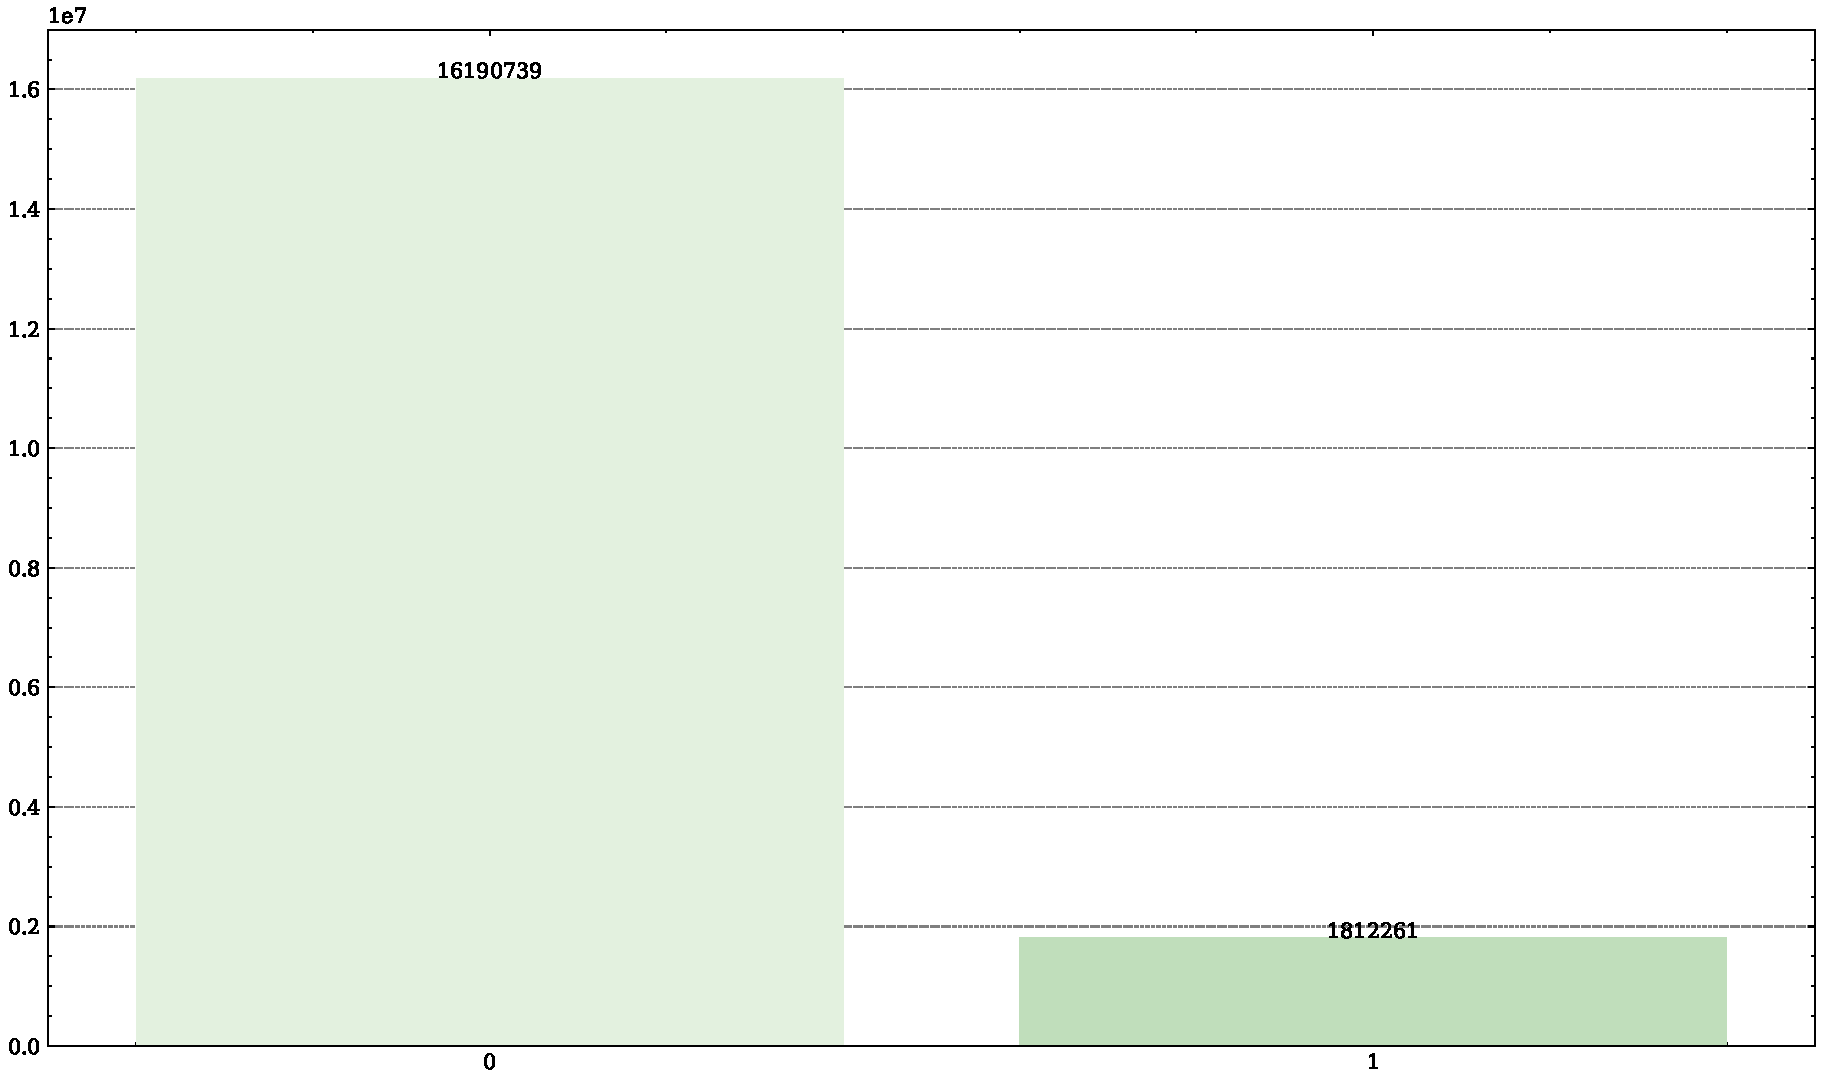
\includegraphics[scale=0.25]{../images/训练集数据个数分布图.pdf}
% 	  \end{minipage}
% 	  \begin{minipage}[t]{0.5\linewidth}
% 		  \centering
% 		  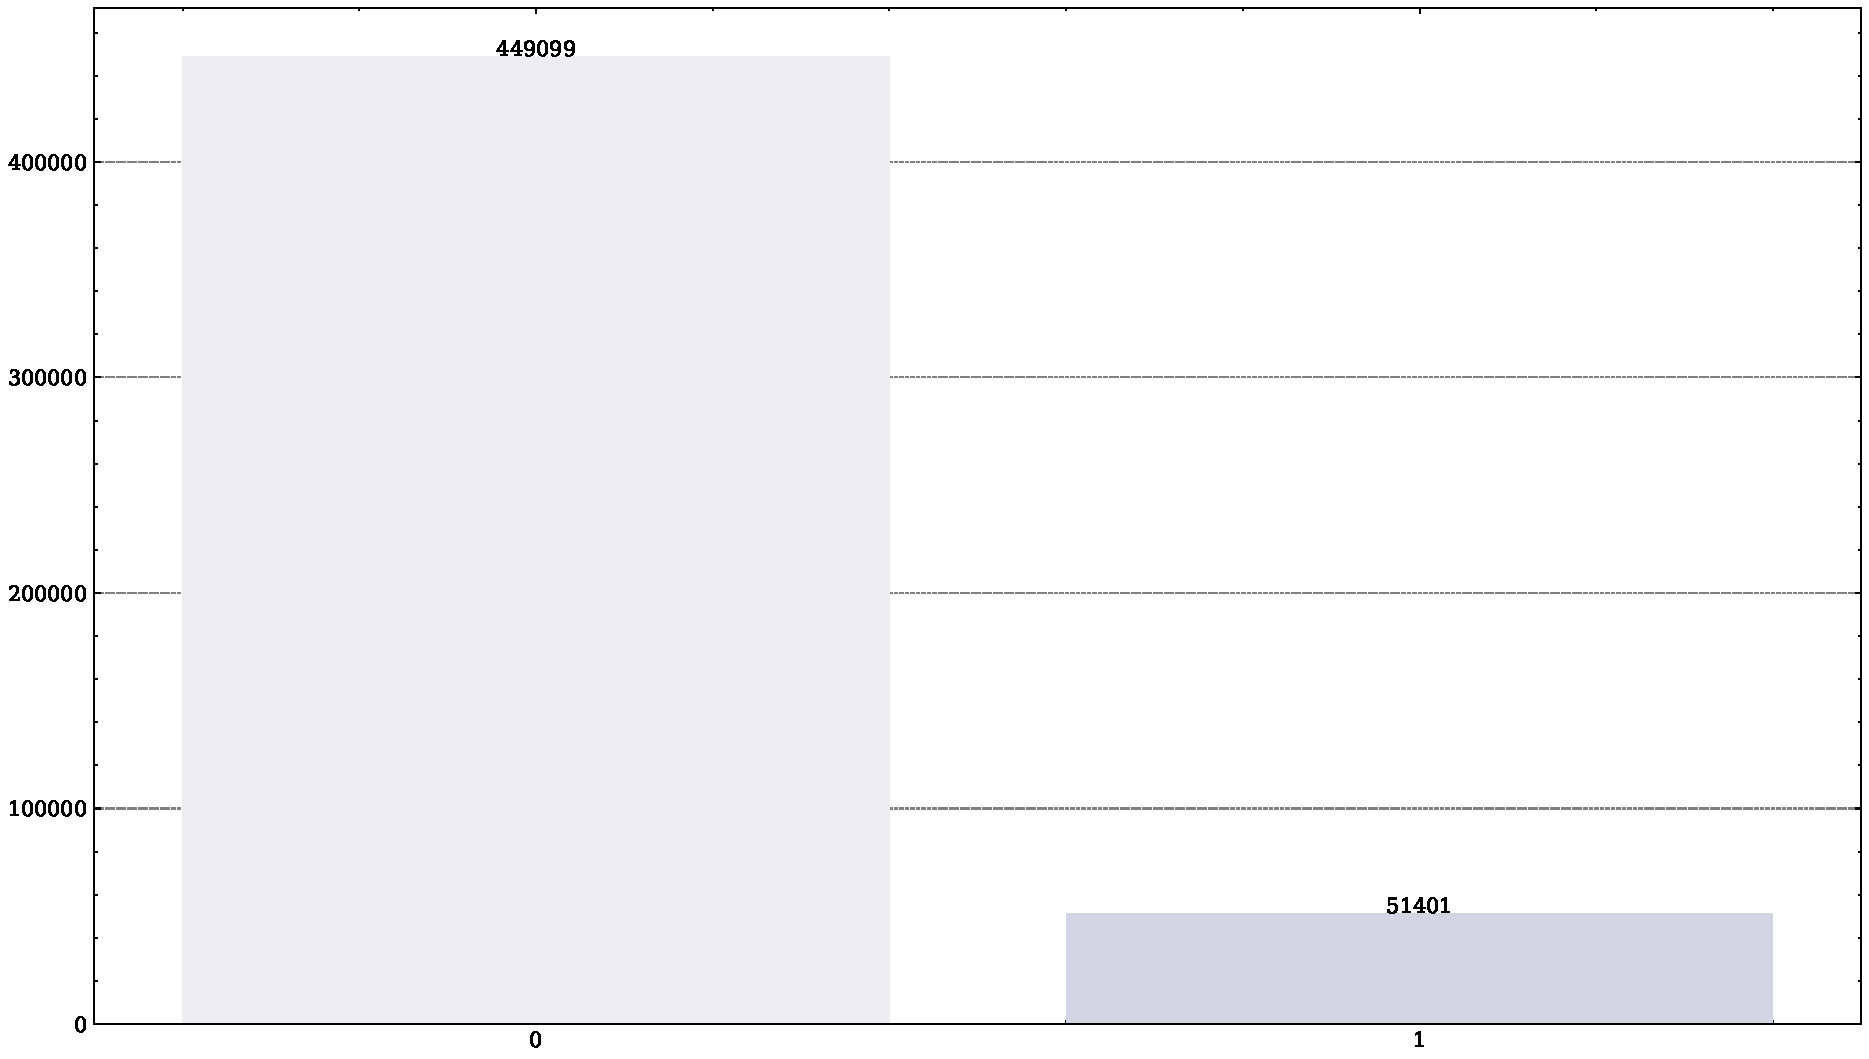
\includegraphics[scale=0.25]{../images/验证集数据个数分布图.pdf}
% 	  \end{minipage}
% 	\caption{数据个数分布图}
% 	\label{数据个数分布图}
% \end{figure}
\begin{figure}[H]
	\begin{center}
		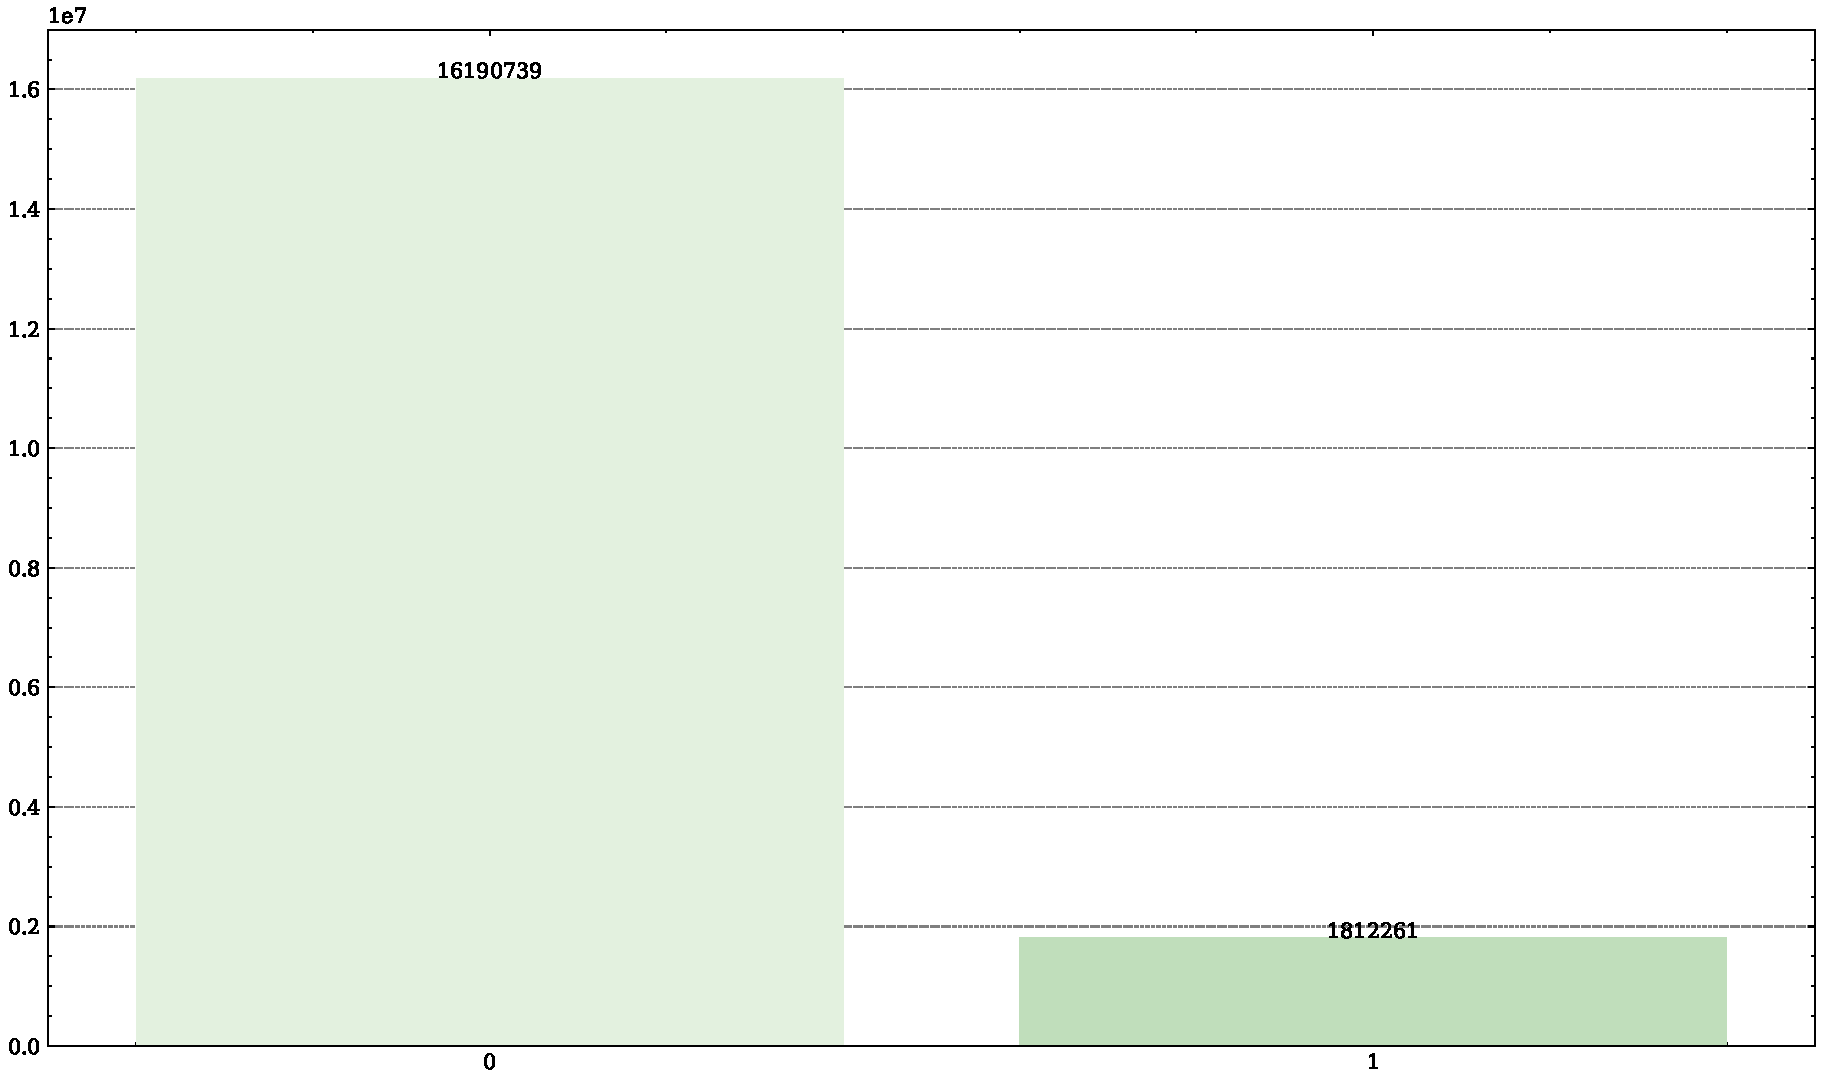
\includegraphics[scale=0.4]{../images/训练集数据个数分布图.pdf}
		\caption{训练集数据个数分布图}
		\label{训练集数据个数分布图}
	\end{center}
\end{figure}
\begin{figure}[H]
	\begin{center}
		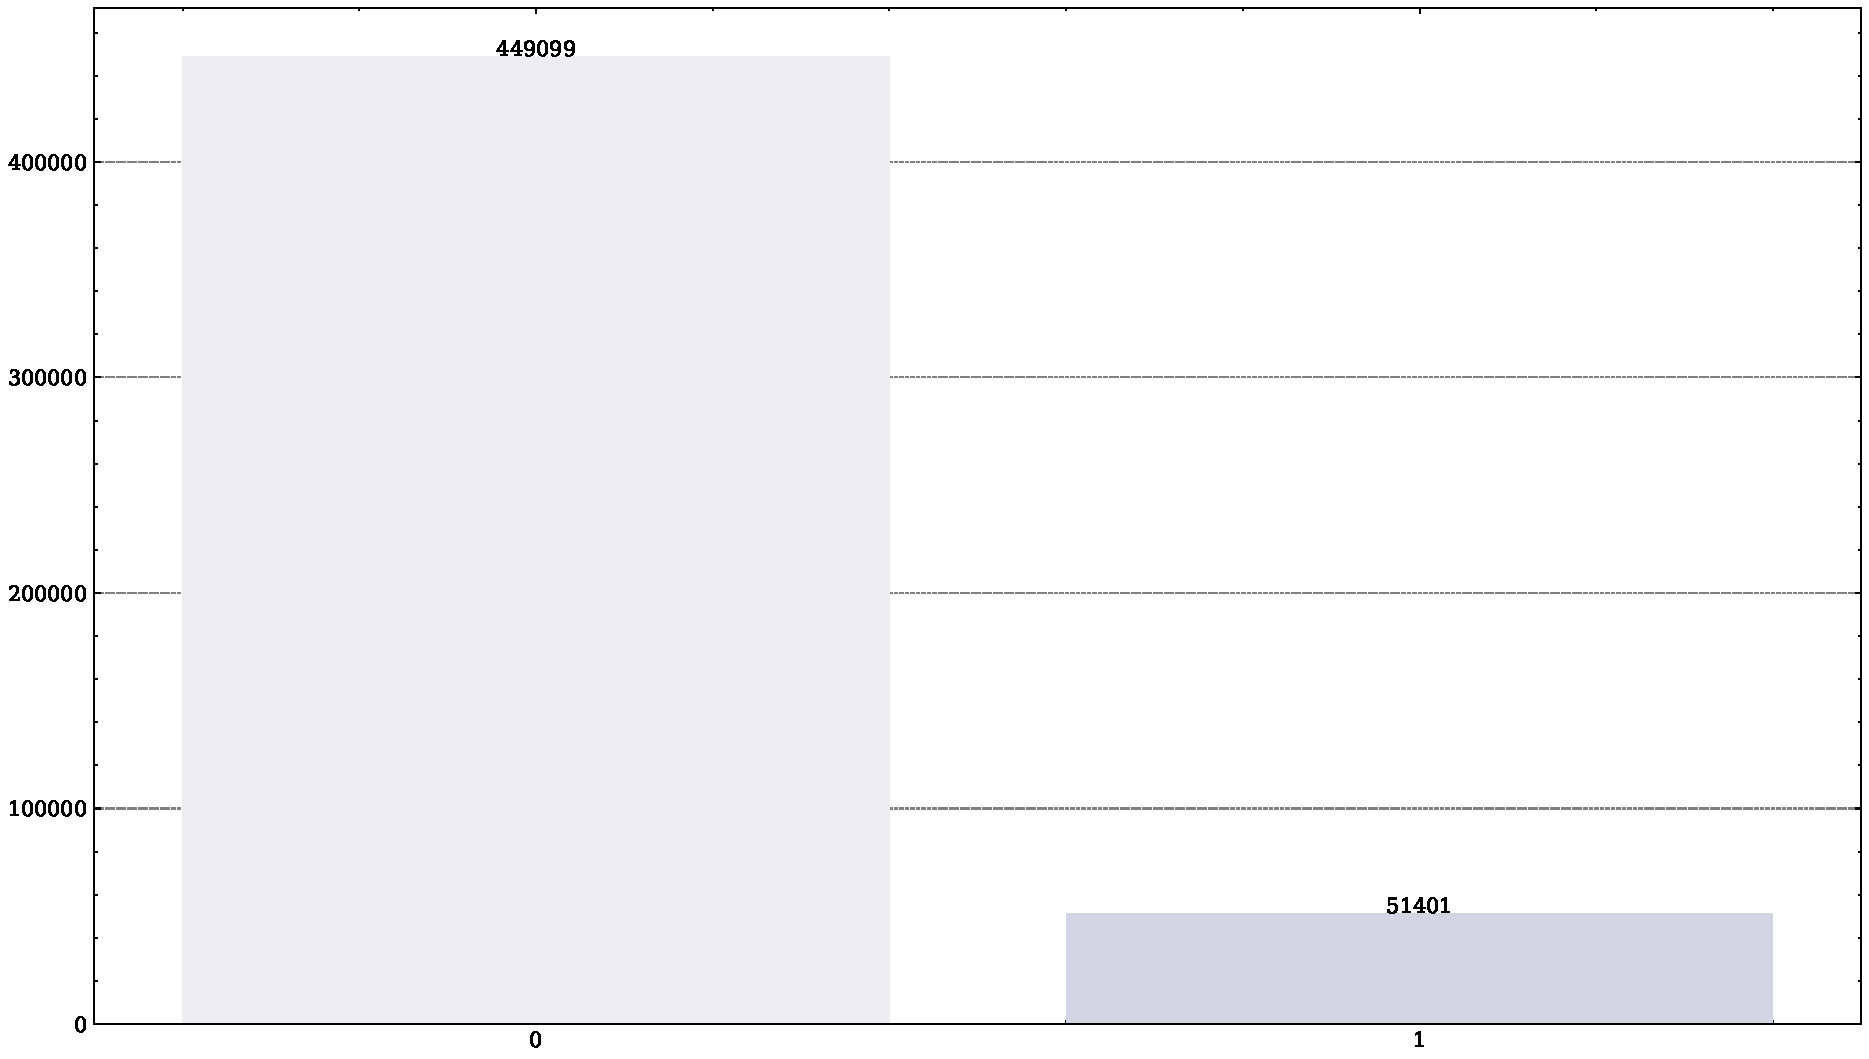
\includegraphics[scale=0.4]{../images/验证集数据个数分布图.pdf}
		\caption{验证集数据个数分布图}
		\label{验证集数据个数分布图}
	\end{center}
\end{figure}

解决类别不平衡问题的方法有很多,例如过采样、欠采样、权重调整、数据增强等。在本次实验中,由于数据集非常大,我们采取随机欠采样的方法对
训练集中的负样本进行欠采样。当生成一批数据时,我们以相同的概率选择当前数据的标签,并根据确定的标签到对应的文件里进一步选择图像对。
这样即可保证在训练集中,正负样本的数量大致相同。具体代码请见下一小节。我们不对验证集进行任何方式的欠采样。

由于数据集足够大,我们不对训练集图像做任何数据增强。

\subsection{Dataset 的构建}
最后,我们编写了一个支持迭代的数据集类,用于将上述数据集转换成可输入模型的形式。这个类的实例在读取训练集时,在每次迭代过程中,
会首先按照上一小节中介绍的方法确定当前要读取的样本的类别。接着会到对应的txt 文件中读取一行。
提取这一行中图片对的地址并找到这两个图像,将两个图像转为 tensor 并在通道维度上合并,最终返回合并后的图像和标签的二元组。
类的实例在读取验证集时,会依次读取验证集的两个 \texttt{txt} 文件中的内容,其余步骤和读取训练集相同。
\texttt{Dataset} 构建的部分核心代码如下。
\begin{lstlisting}
class DigitsDataset(Dataset):
    def __init__(self, info_names: tuple[str], is_train:bool, transform=None):
		"""
		:params info_names: 元组,两种标签文件的路径
		:params is_train: 是否是训练集
		:params transform: 数据增强函数,默认无数据增强 (None)
		"""
        super().__init__()
        set_seed(params["random_seed"])
        self.train = is_train
        self.data_info_0 = self.get_img_info(info_names[0]) # 所有标签为 0 的图像对
        self.data_info_1 = self.get_img_info(info_names[1]) # 所有标签为 1 的图像对
        random.shuffle(self.data_info_0)
        random.shuffle(self.data_info_1)
        self.transform = transform

	def __getitem__(self, index):
		if self.train: # 读取训练集数据
			if random.random() < params["dataset_thres"]: # 当前数据选择标签 0
				data_info = self.data_info_0
				label = 0
			else: # 当前数据选择标签 0
				data_info = self.data_info_1
				label = 1
			path_img1, path_img2 = data_info[index]
		else: # 读取验证集数据
			if index < len(self.data_info_0): # 正在读取负样本
				path_img1, path_img2 = self.data_info_0[index]
				label = 0
			else: # 正在读取正样本
				path_img1, path_img2 = self.data_info_1[index - len(self.data_info_0)]
				label = 1
		
		img1, img2 = Image.open(path_img1), Image.open(path_img2)
		if self.transform is not None:
			img1, img2 = self.transform(img1), self.transform(img2)

		return torch.cat((img1, img2), dim=0), label
	
	def __len__(self):
		if self.train: # 训练集长度
			return len(self.data_info_1)
		else: # 验证集长度
			return len(self.data_info_0) + len(self.data_info_1)
\end{lstlisting}

至此,数据处理完成。

\section{模型架构}
接下来,我们进行模型架构的设计。在本实验中,我们一共设计了两个模型架构,并均进行了测试。
\subsection{网络结构}
根据实验要求,网络应为一个包含残差块的卷积神经网络。我们设计了两种带有残差块的网络架构。它们分别是 LeNet\_RB 和 ResNet18。
下面,我们首先介绍残差块的结构,再分别介绍两种网络的结构。

残差块包括两个分支:left 和 shortcut。其中,left 分支由两个卷积层、两个批归一化层和一个 ReLU 激活函数层组成。
shortcut 分支由一个卷积层和一个批归一化层。层的输出是输入经两个分支映射后的结果之和。残差块的结构如图\ref{残差块网络结构图}
所示。
\begin{figure}[H]
	\begin{center}
		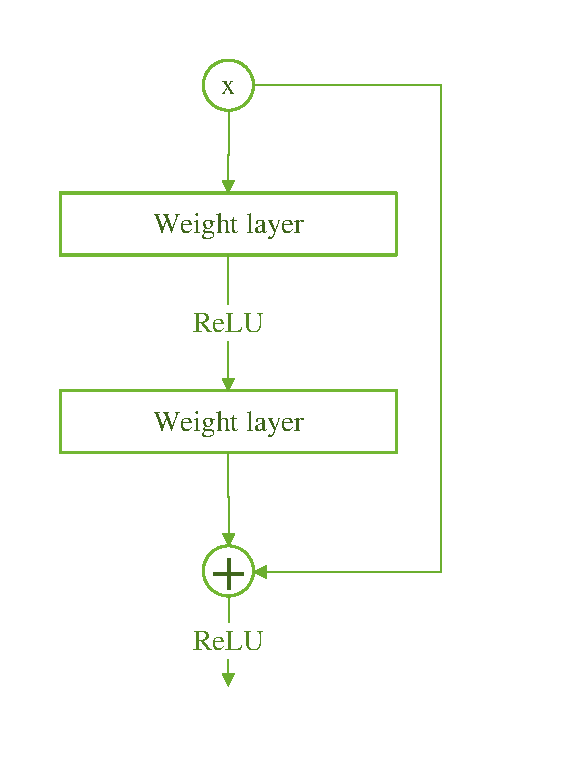
\includegraphics[scale=0.7]{../images/残差块网络结构图.pdf}
		\caption{残差块网络结构图}
		\label{残差块网络结构图}
	\end{center}
\end{figure}

LeNet\_RB 是 LeNet5 网络和一个残差块组成的。我们将一个残差块放到 LeNet5 的卷积层和全连接层之间,即可得到 LeNet\_RB。
LeNet\_RB 的网络结构图如图\ref{LeNetRB网络结构图}所示。该网络的参数较少,所以训练时间和推理时间较短,适合于简单的图像分类任务。
\begin{figure}[H]
	\begin{center}
		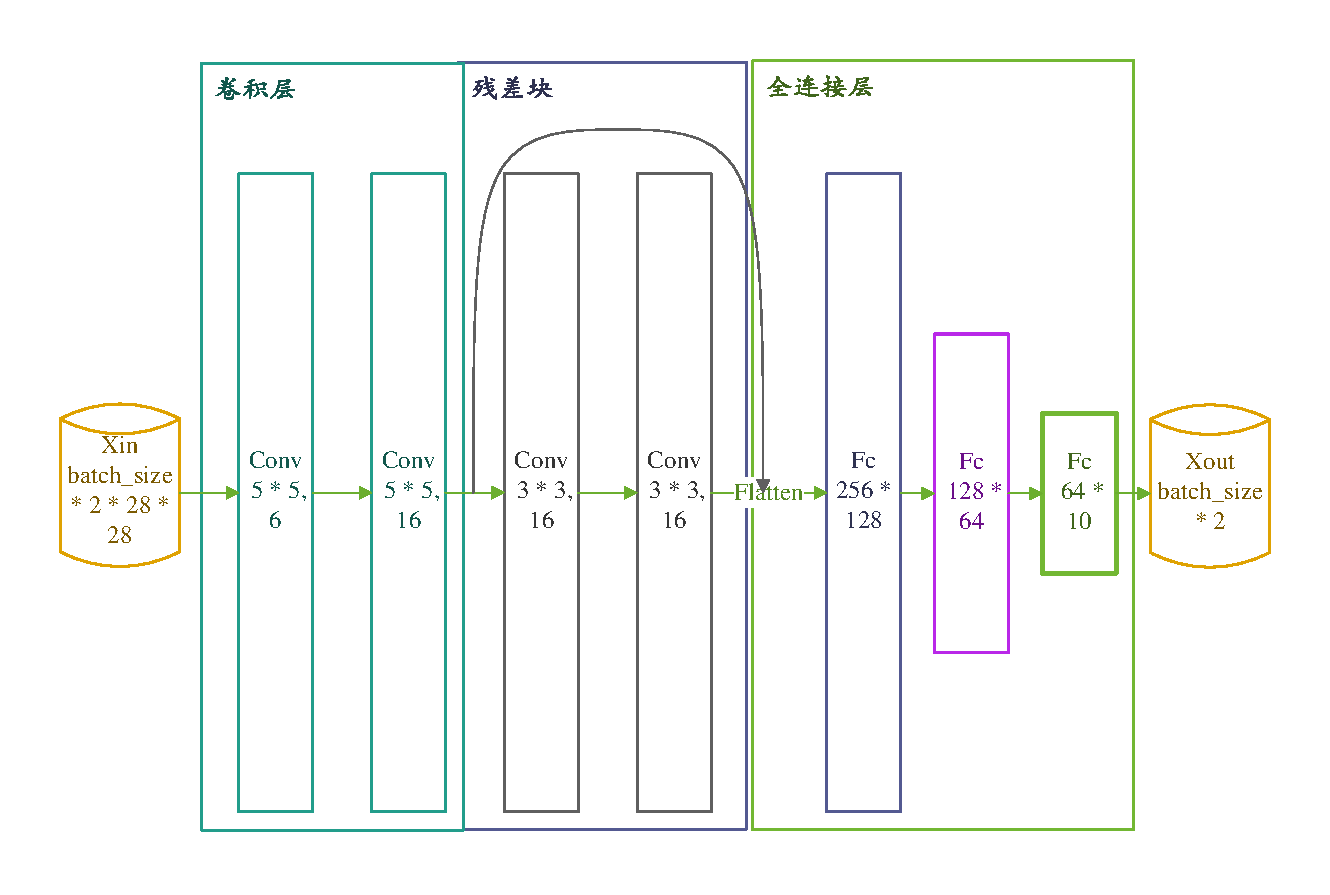
\includegraphics[scale=0.45]{../images/LeNetRB网络结构图.pdf}
		\caption{LeNet\_RB 网络结构图}
		\label{LeNetRB网络结构图}
	\end{center}
\end{figure}

ResNet18 是 ResNet 的最小版本,它由 18 个层组成。ResNet18 包含 1 个卷积层、4 个残差连接层、1个池化层和 1 个全连接层。其中, 1 个残差连接层由 2 个残差块连接而成。
ResNet18 的网络结构图如图\ref{ResNet18网络结构图}所示。该网络的参数较多,可以本实验中达到更高的准确率,但是训练和推理时间较长。
\begin{figure}[H]
	\begin{center}
		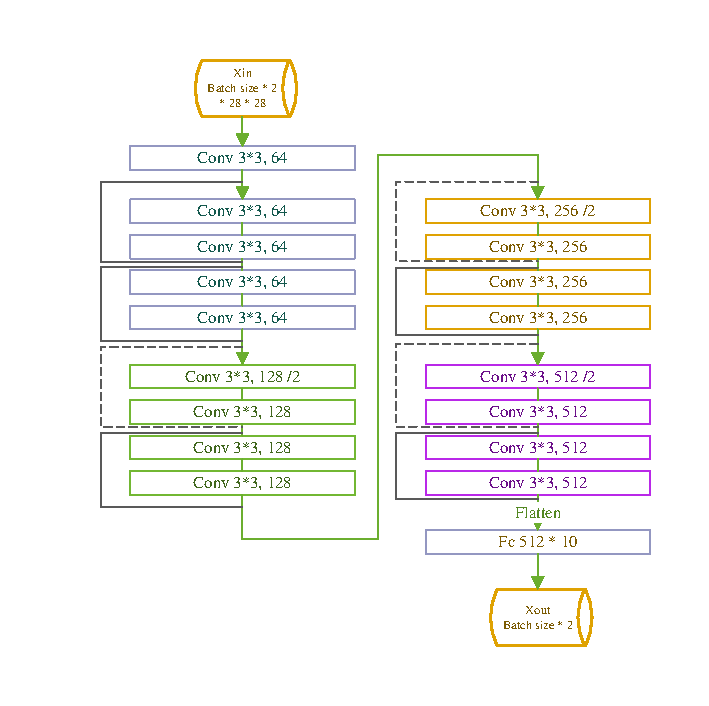
\includegraphics[scale=0.9]{../images/ResNet18网络结构图.pdf}
		\caption{ResNet18 网络结构图}
		\label{ResNet18网络结构图}
	\end{center}
\end{figure}

\subsection{损失函数}
损失函数是度量当前分类器的输出和真实值的差异的函数。
本实验要求完成一个二分类任务。所以,我们使用交叉熵损失来作为我们的损失函数。
交叉熵是一种在分类任务中常用的损失函数。假设分类器的输出向量 $p\in R^c$,
真实值的独热向量为 $q\in R^c$。那么交叉熵 $H(p, q)$ 的计算公式如下。
$$
H(p, q)=-\sum_{i=1}^{c}p_i log(q_i)
$$

\subsection{优化器}
优化器用来决定下一步模型的参数如何变化。在本实验中,我们选用 AdamW 优化器。
AdamW 优化器是 Adam 优化器的改进版本。它在 Adam 优化器的基础上增加了权值衰减功能。
Adam 优化器同时考虑指数移动平均的一阶动量和二阶动量以指导参数更新。其计算公式如下。
$$
\begin{aligned}
	m_t&=\beta_1m_{t-1}+(1-\beta_1)g_t\\
	v_t&=\beta_2v_{t-1}+(1-\beta_2)diag(g_t^2)\\
	w_{t+1}&=w_{t}-\alpha\frac{m_t}{\sqrt{v_t}+\epsilon}
\end{aligned}
$$

其中,$m_t, v_t$ 是动量相关参数,$\alpha$ 为学习率,$w_t$ 是参数矩阵,$g_t$ 是梯度。
而 Adamw 优化器在 Adam 优化器的基础上加入了权值衰减系数,$w$ 矩阵的更新公式变为。
$$
w_{t+1}=(1-\lambda \alpha)w_{t}-\alpha\frac{m_t}{\sqrt{v_t}+\epsilon}
$$

由于 AdamW 优化器已经进行了学习率自适应,在本次实验中我们向优化器中传入固定值的学习率,而不在设置
学习率更新策略,使其随训练轮数发生变化。

至此,网络架构设计完成。


\section{实验结果}
\subsection{实验环境}
本实验在一个运算服务器上进行,服务器的配置如表\ref{服务器配置}所示。
\begin{table}[H]
	\centering
	\caption{实验环境表}
	  \begin{tabular}{c|c|c}
		\toprule
	  \multirow{3}[0]{*}{硬件} & CPU   & AMD EPYC 7551P 32-Core Processor \\
			& 内存大小    & 440G \\
			& GPU   & NVIDIA GeForce RTX 3090 \\\hline
	  \multirow{3}[0]{*}{软件} & 操作系统  & Ubuntu 20.04.5 LTS \\
			& 深度学习框架 & PyTorch 1.13.1 \\
			& IDE   & Vscode \\\bottomrule
	  \end{tabular}
	\label{服务器配置}
\end{table}
\subsection{超参数设置}
在本次实验中,为了使结果可复现,我们将随机数种子固定为 1024。我们还使用了 GPU 加速训练。

在网络架构方面,我们训练了 LeNet\_RB, ResNet18 两种模型。模型的架构已在上文中介绍。两种模型的输入均为一批 $28\times 28\times 2$
的矩阵,输出为相同数量的预测标签。

对于优化器,我们选择了 AdamW 优化器,$\beta_1$ 参数为 0.9,$\beta_2$ 参数为 0.999。

在训练方面,对于 LeNet\_RB 模型。我们训练 30 个 epoch,将 batch size 设置成 10000,学习率设置成 $5\times 10^{-3}$。
对于 ResNet18 模型。我们训练 30 个 epoch,将 batch size 设置成 4000,学习率设置成 0.01。

\subsection{结果}
首先,我们使用上述的超参数对模型进行了训练,在完成每一轮训练后我们将模型在验证集上进行验证。验证所使用的评价指标
包括准确率和 f1 分数。我们选择验证集上准确率最高的模型参数进行保存。

% here
在训练过程中,对于 LeNet\_RB模型,每个 mini\_batch 上训练集损失函数值变化和评价指标变化
如图\ref{LeNetRB训练损失函数batch}和图\ref{LeNetRB训练评价指标batch}所示;
每个 epoch 结束后训练集和验证集上的损失函数如图\ref{LeNetRB训练验证损失函数}所示;
每个 epoch 结束后训练集和验证集上的评价指标(准确率和 f1 分数)如图\ref{LeNetRB训练验证acc}和图\ref{LeNetRB训练验证f1}所示。
\begin{figure}[H]
	\begin{center}
		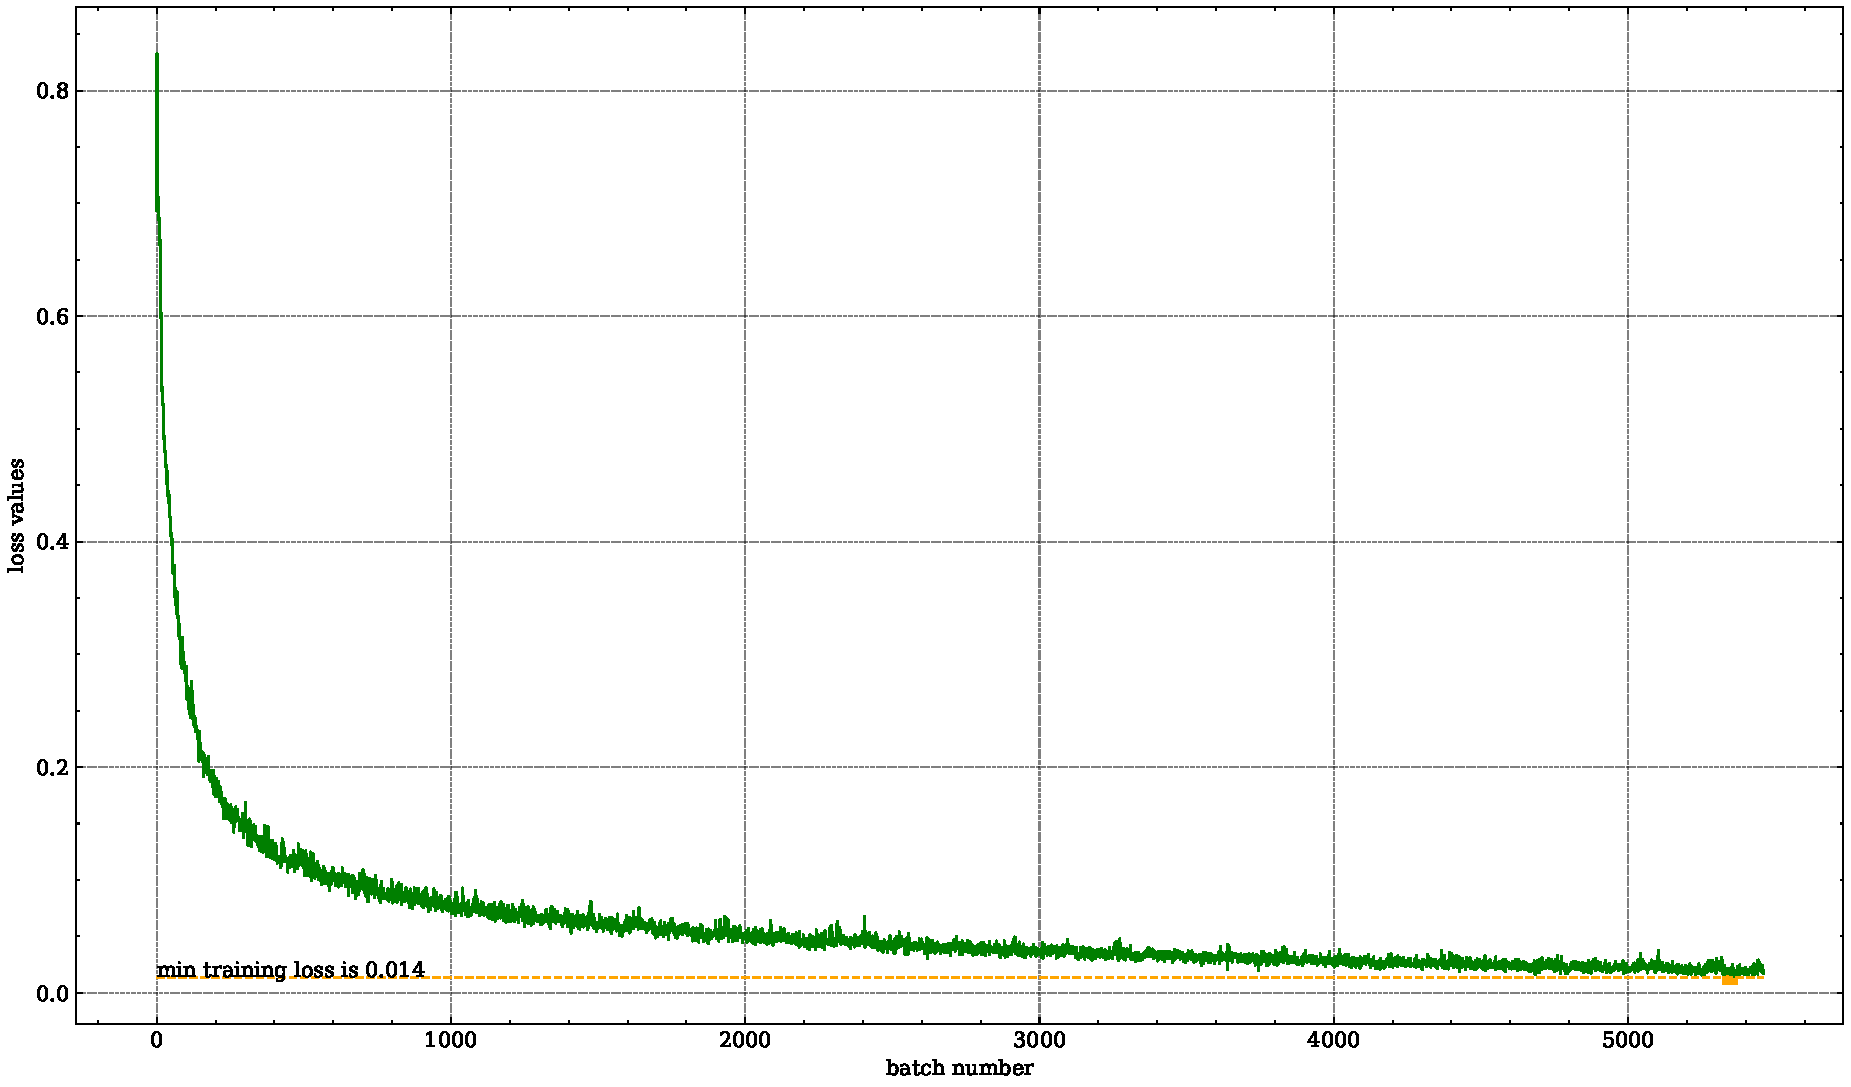
\includegraphics[scale=0.45]{../images/LeNetRB训练损失函数batch.pdf}
		\caption{LeNet\_RB训练损失函数变化图}
		\label{LeNetRB训练损失函数batch}
	\end{center}
\end{figure}
\begin{figure}[H]
	\begin{center}
		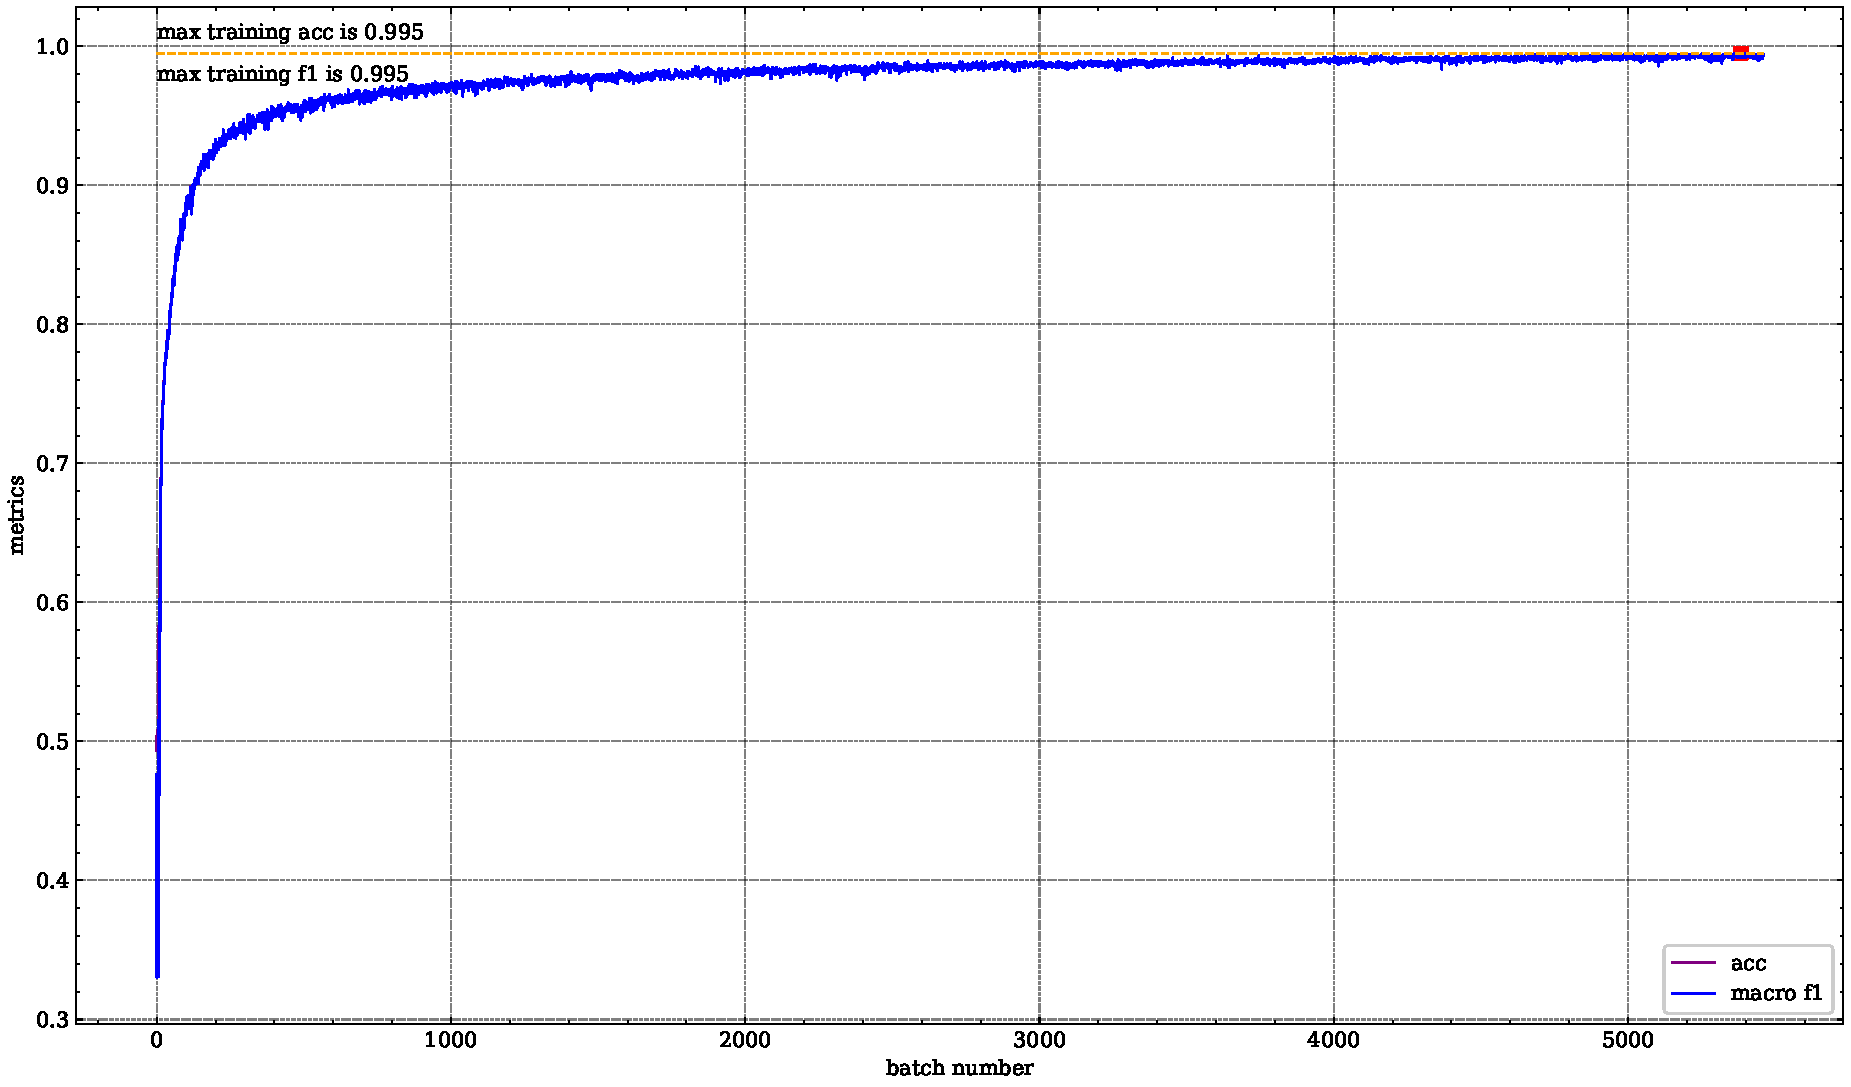
\includegraphics[scale=0.45]{../images/LeNetRB训练评价指标batch.pdf}
		\caption{LeNet\_RB训练评价指标变化图}
		\label{LeNetRB训练评价指标batch}
	\end{center}
\end{figure}
\begin{figure}[H]
	\begin{center}
		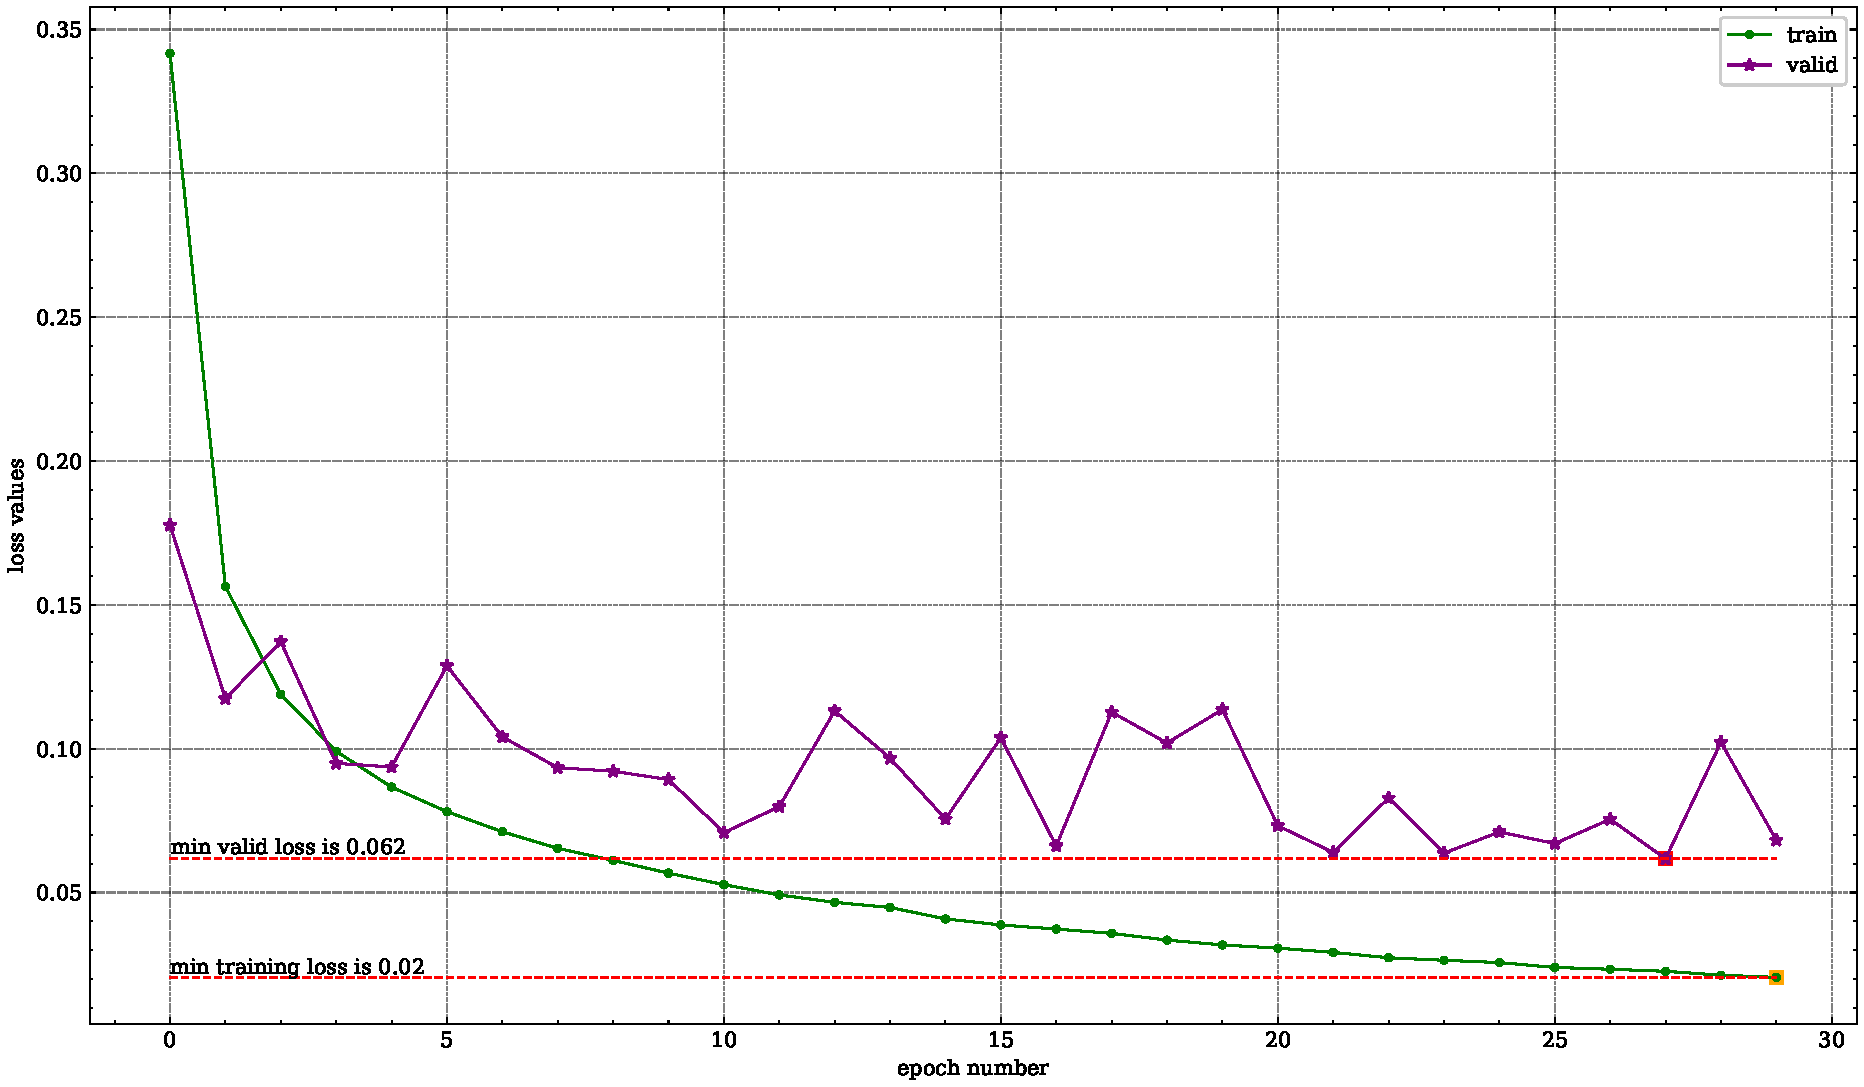
\includegraphics[scale=0.45]{../images/LeNetRB训练验证损失函数.pdf}
		\caption{LeNet\_RB 训练损失函数变化图}
		\label{LeNetRB训练验证损失函数}
	\end{center}
\end{figure}
\begin{figure}[H]
	\begin{center}
		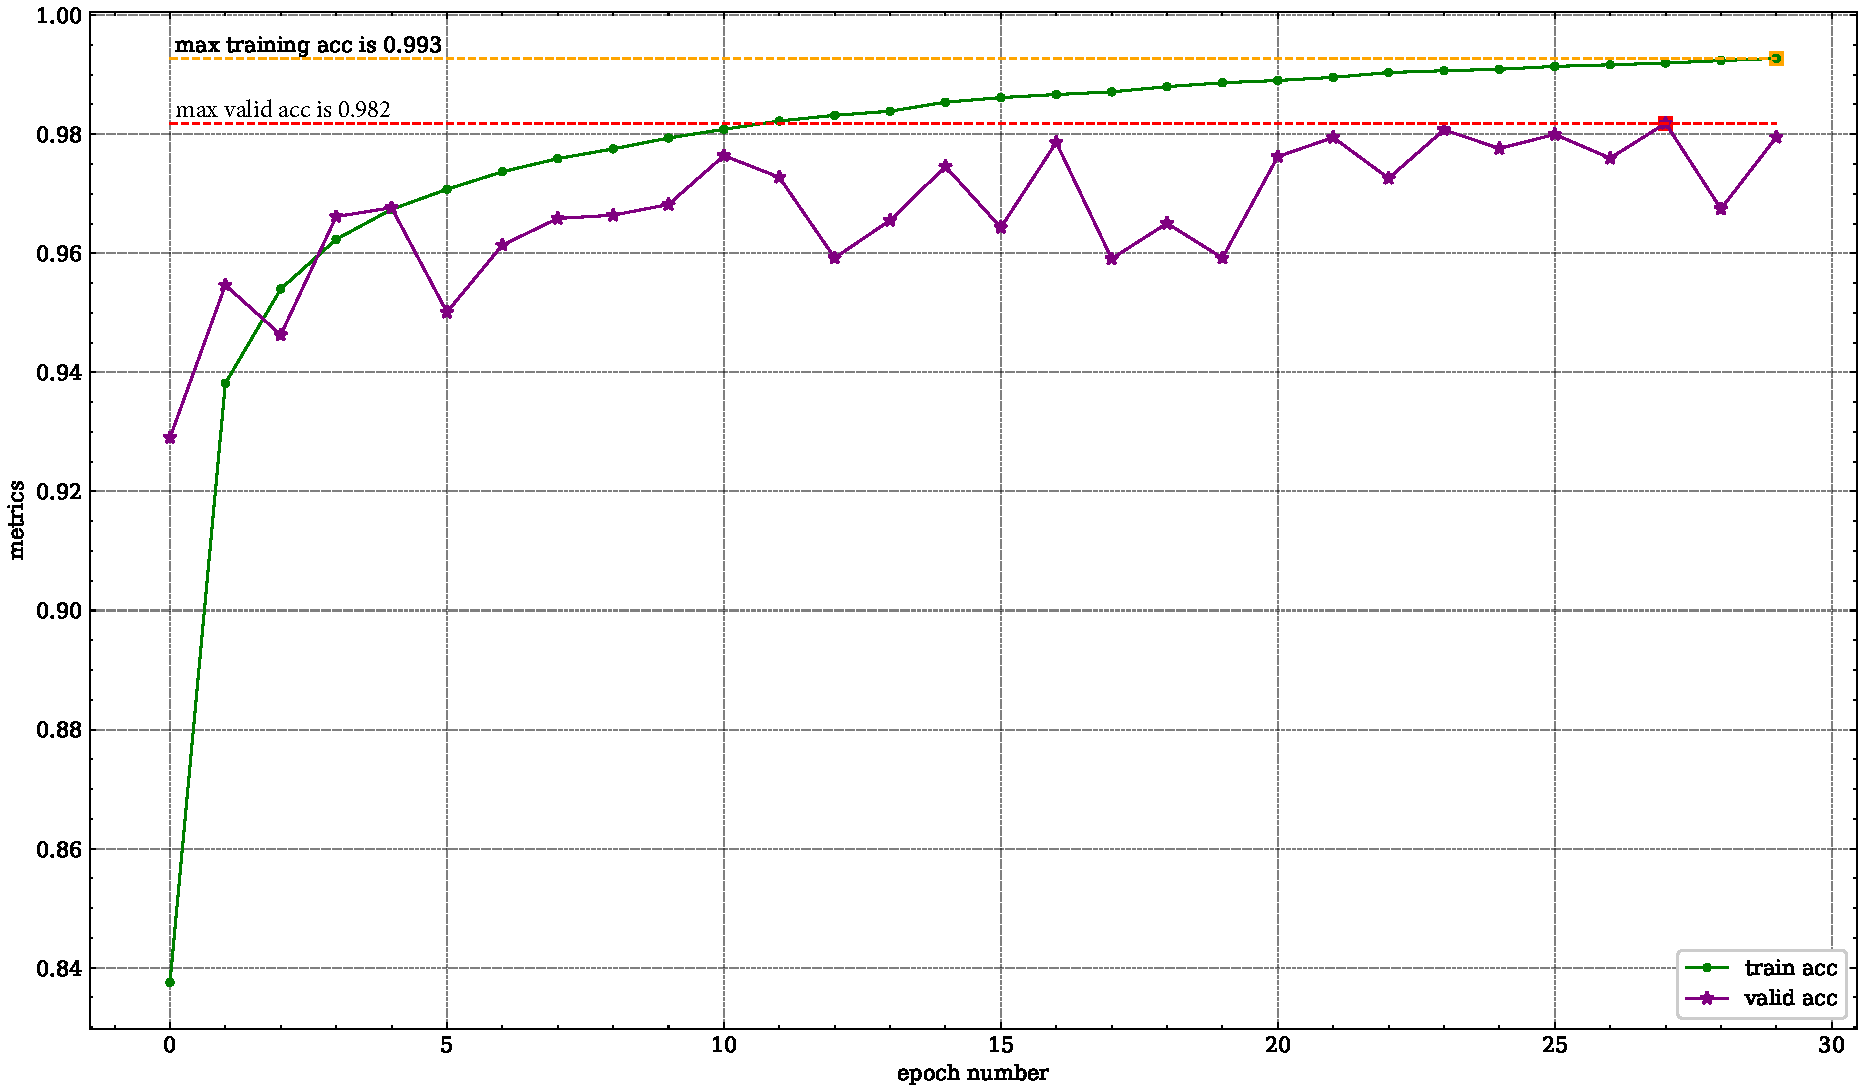
\includegraphics[scale=0.45]{../images/LeNetRB训练验证acc.pdf}
		\caption{LeNet\_RB 验证准确率变化图}
		\label{LeNetRB训练验证acc}
	\end{center}
\end{figure}
\begin{figure}[H]
	\begin{center}
		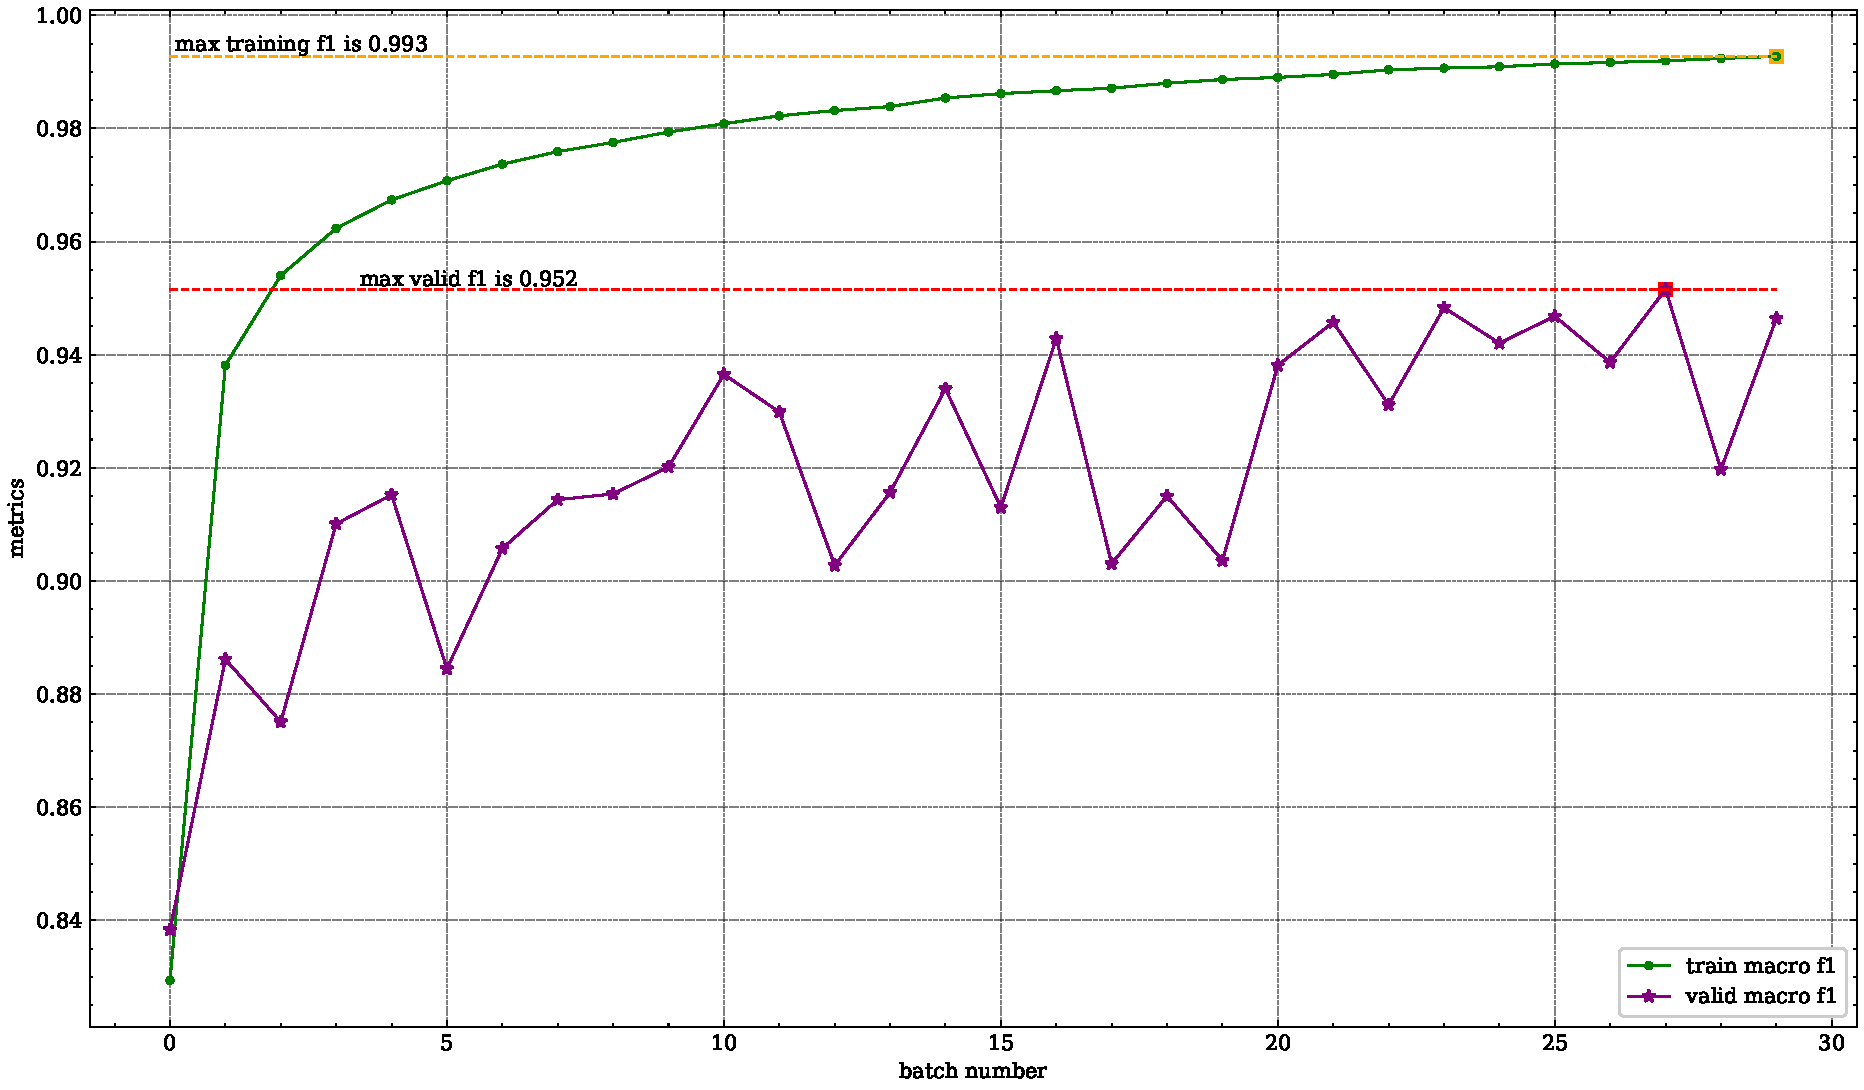
\includegraphics[scale=0.45]{../images/LeNetRB训练验证f1.pdf}
		\caption{LeNet\_RB 验证 f1 分数变化图}
		\label{LeNetRB训练验证f1}
	\end{center}
\end{figure}

对于 ResNet18 模型,每个 mini\_batch 上训练集损失函数值变化和评价指标变化
如图\ref{ResNet18训练损失函数batch}和图\ref{ResNet18训练评价指标batch}所示;
每个 epoch 结束后训练集和验证集上的损失函数如图\ref{ResNet18训练验证损失函数}所示;
每个 epoch 结束后训练集和验证集上的评价指标(准确率和 macro f1 分数)如图\ref{ResNet18训练验证acc}和图\ref{ResNet18训练验证f1}所示。
\begin{figure}[H]
	\begin{center}
		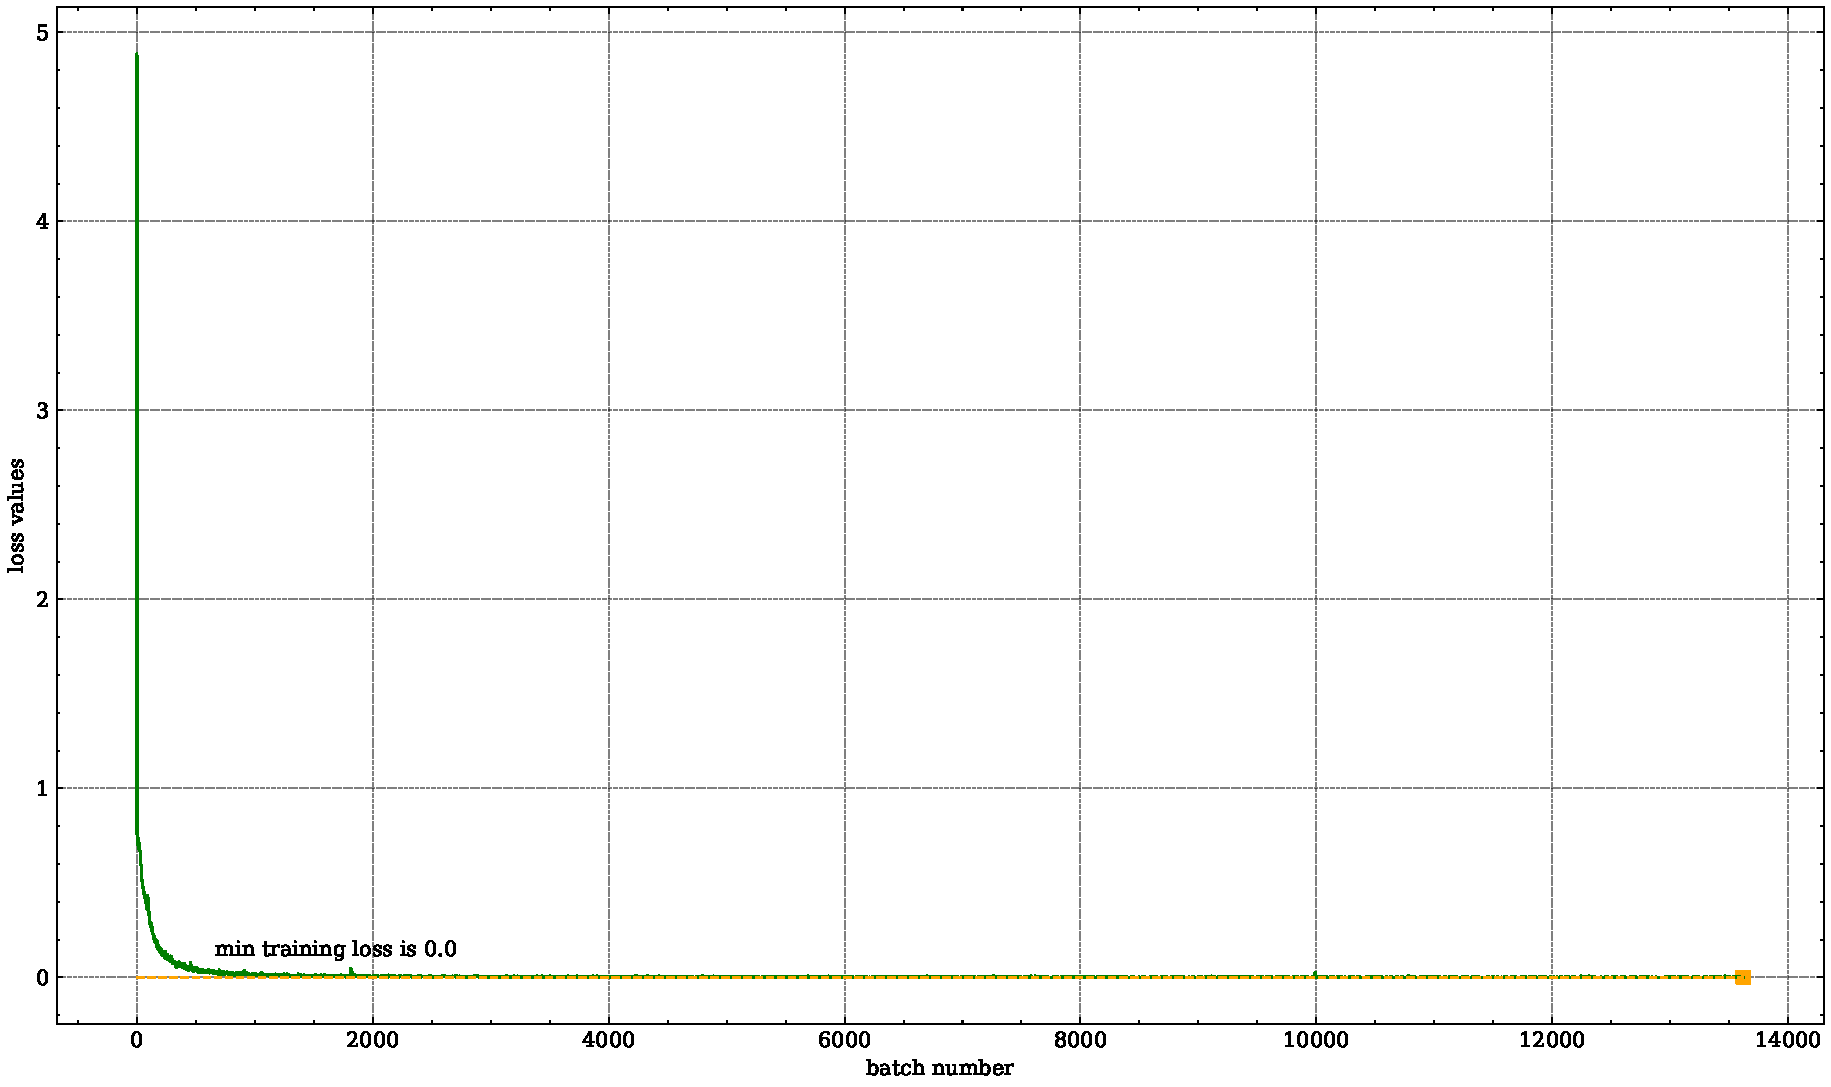
\includegraphics[scale=0.45]{../images/ResNet18训练损失函数batch.pdf}
		\caption{ResNet18训练损失函数变化图}
		\label{ResNet18训练损失函数batch}
	\end{center}
\end{figure}
\begin{figure}[H]
	\begin{center}
		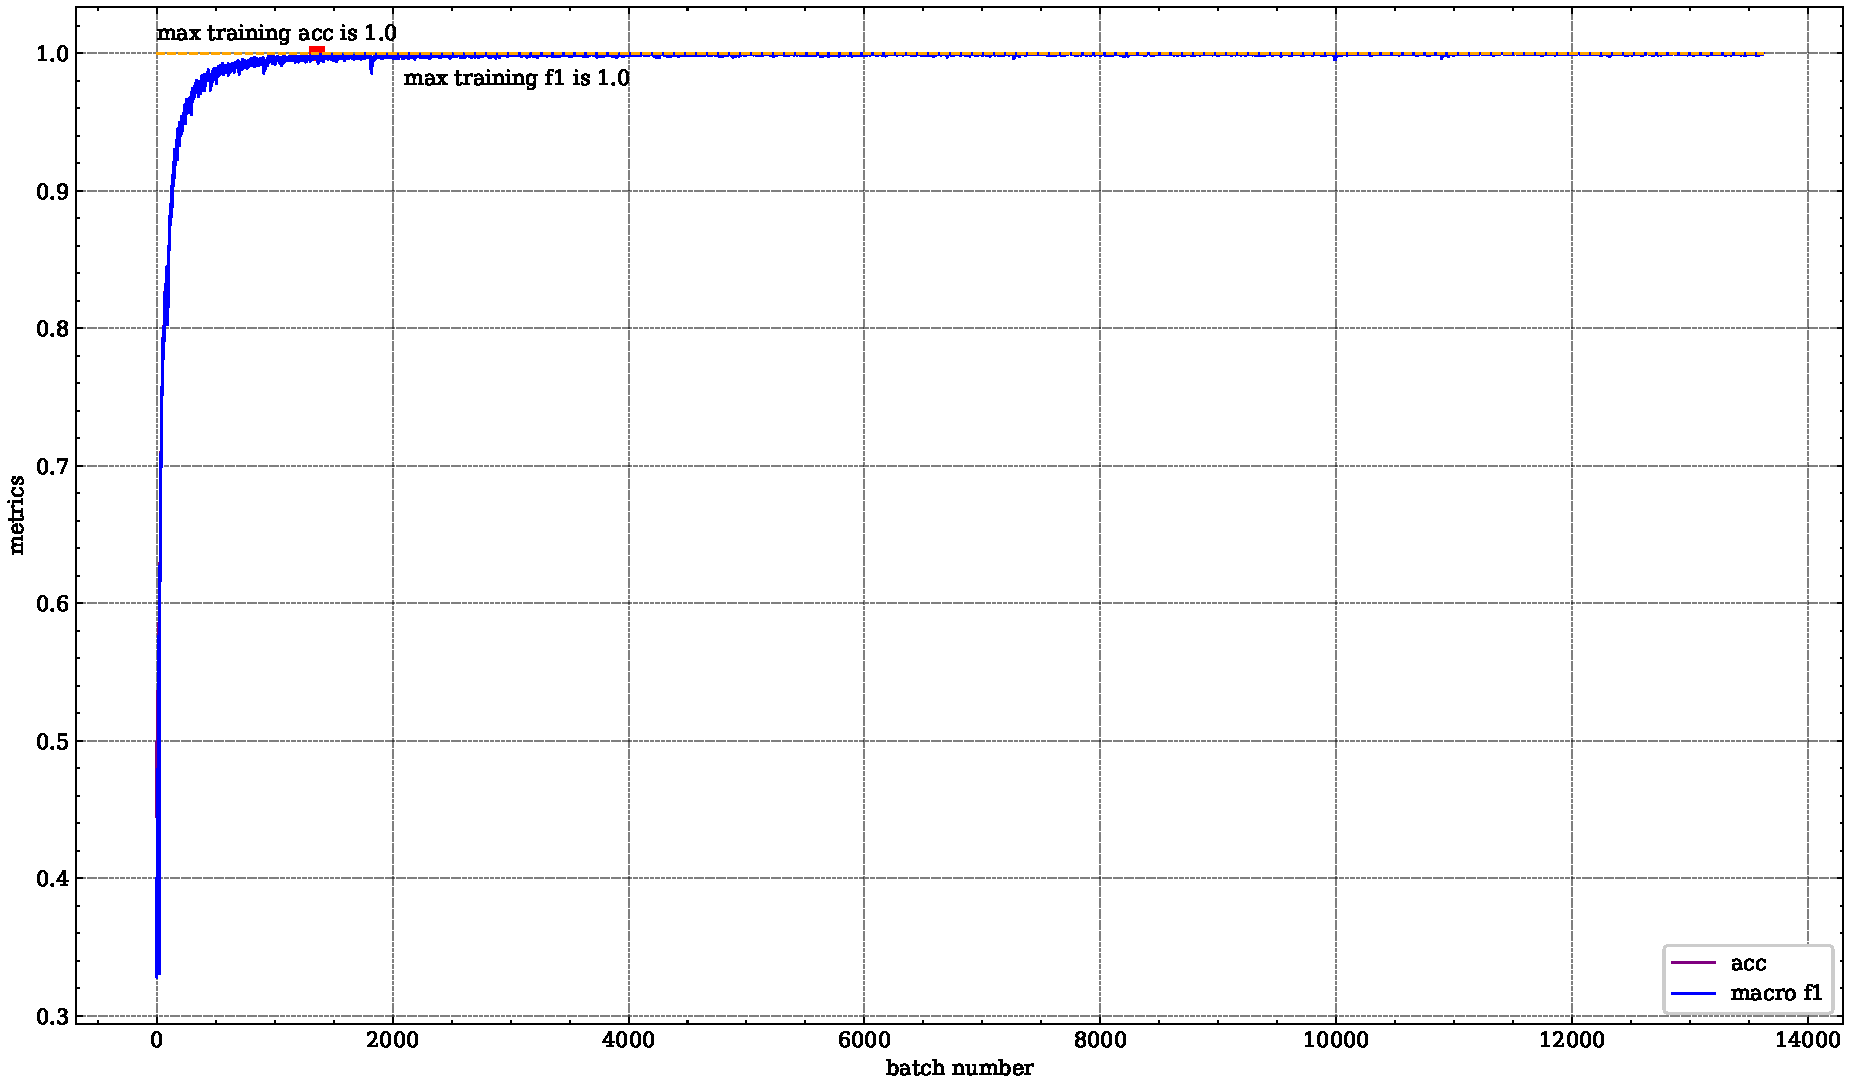
\includegraphics[scale=0.45]{../images/ResNet18训练评价指标batch.pdf}
		\caption{ResNet18训练评价指标变化图}
		\label{ResNet18训练评价指标batch}
	\end{center}
\end{figure}
\begin{figure}[H]
	\begin{center}
		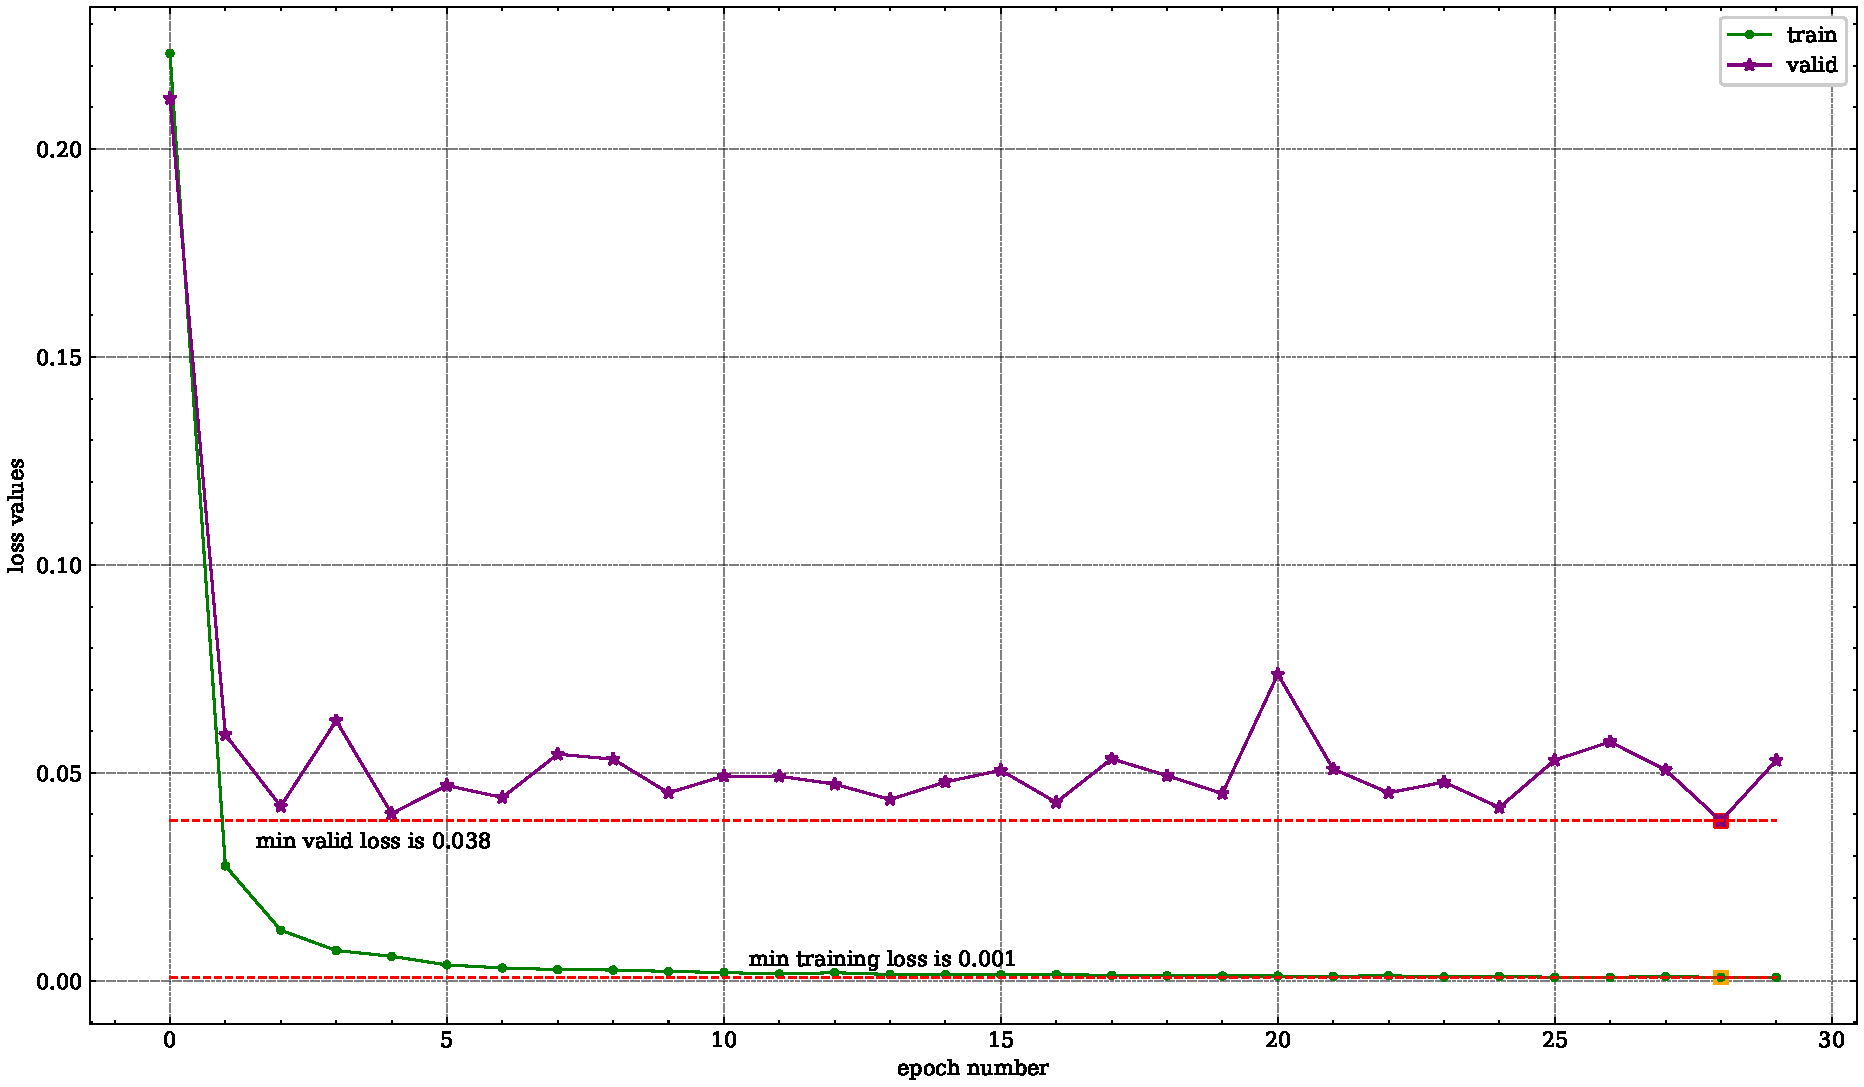
\includegraphics[scale=0.45]{../images/ResNet18训练验证损失函数.pdf}
		\caption{ResNet18 训练损失函数变化图}
		\label{ResNet18训练验证损失函数}
	\end{center}
\end{figure}
\begin{figure}[H]
	\begin{center}
		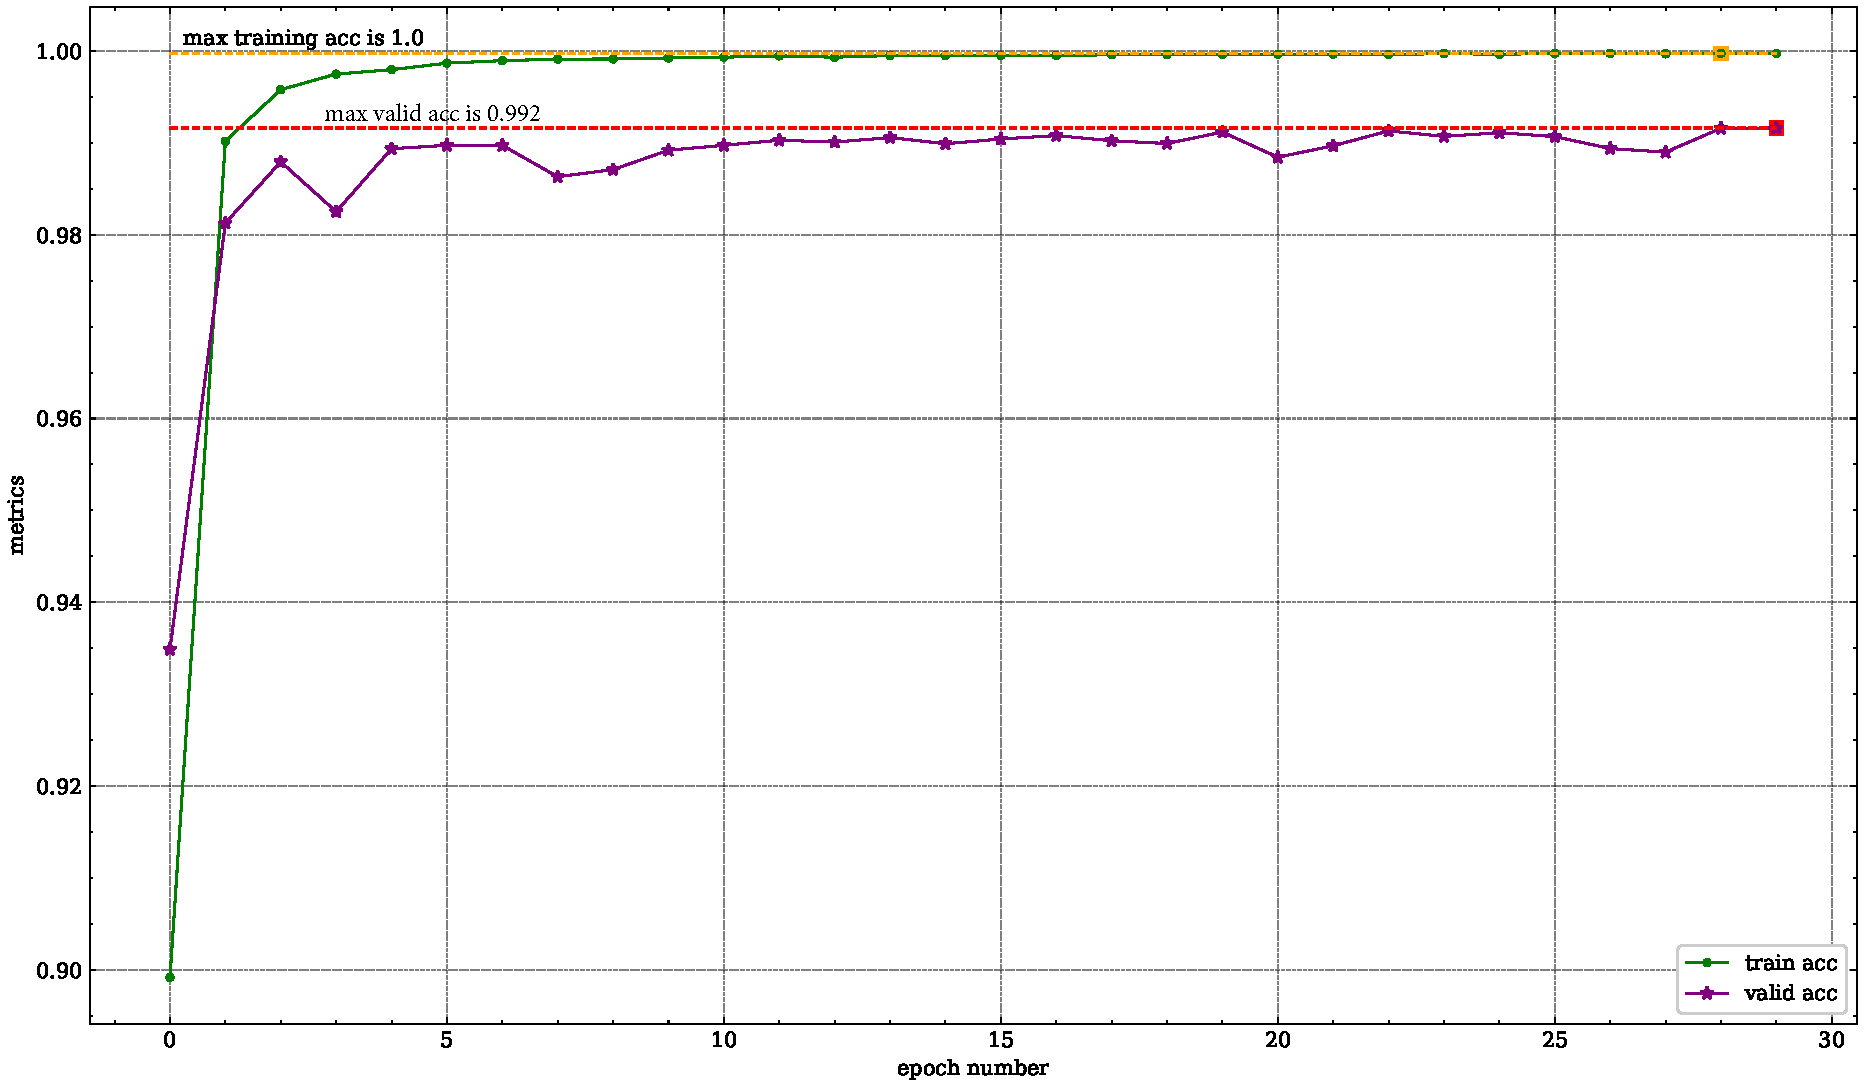
\includegraphics[scale=0.4]{../images/ResNet18训练验证acc.pdf}
		\caption{ResNet18 验证准确率变化图}
		\label{ResNet18训练验证acc}
	\end{center}
\end{figure}
\begin{figure}[H]
	\begin{center}
		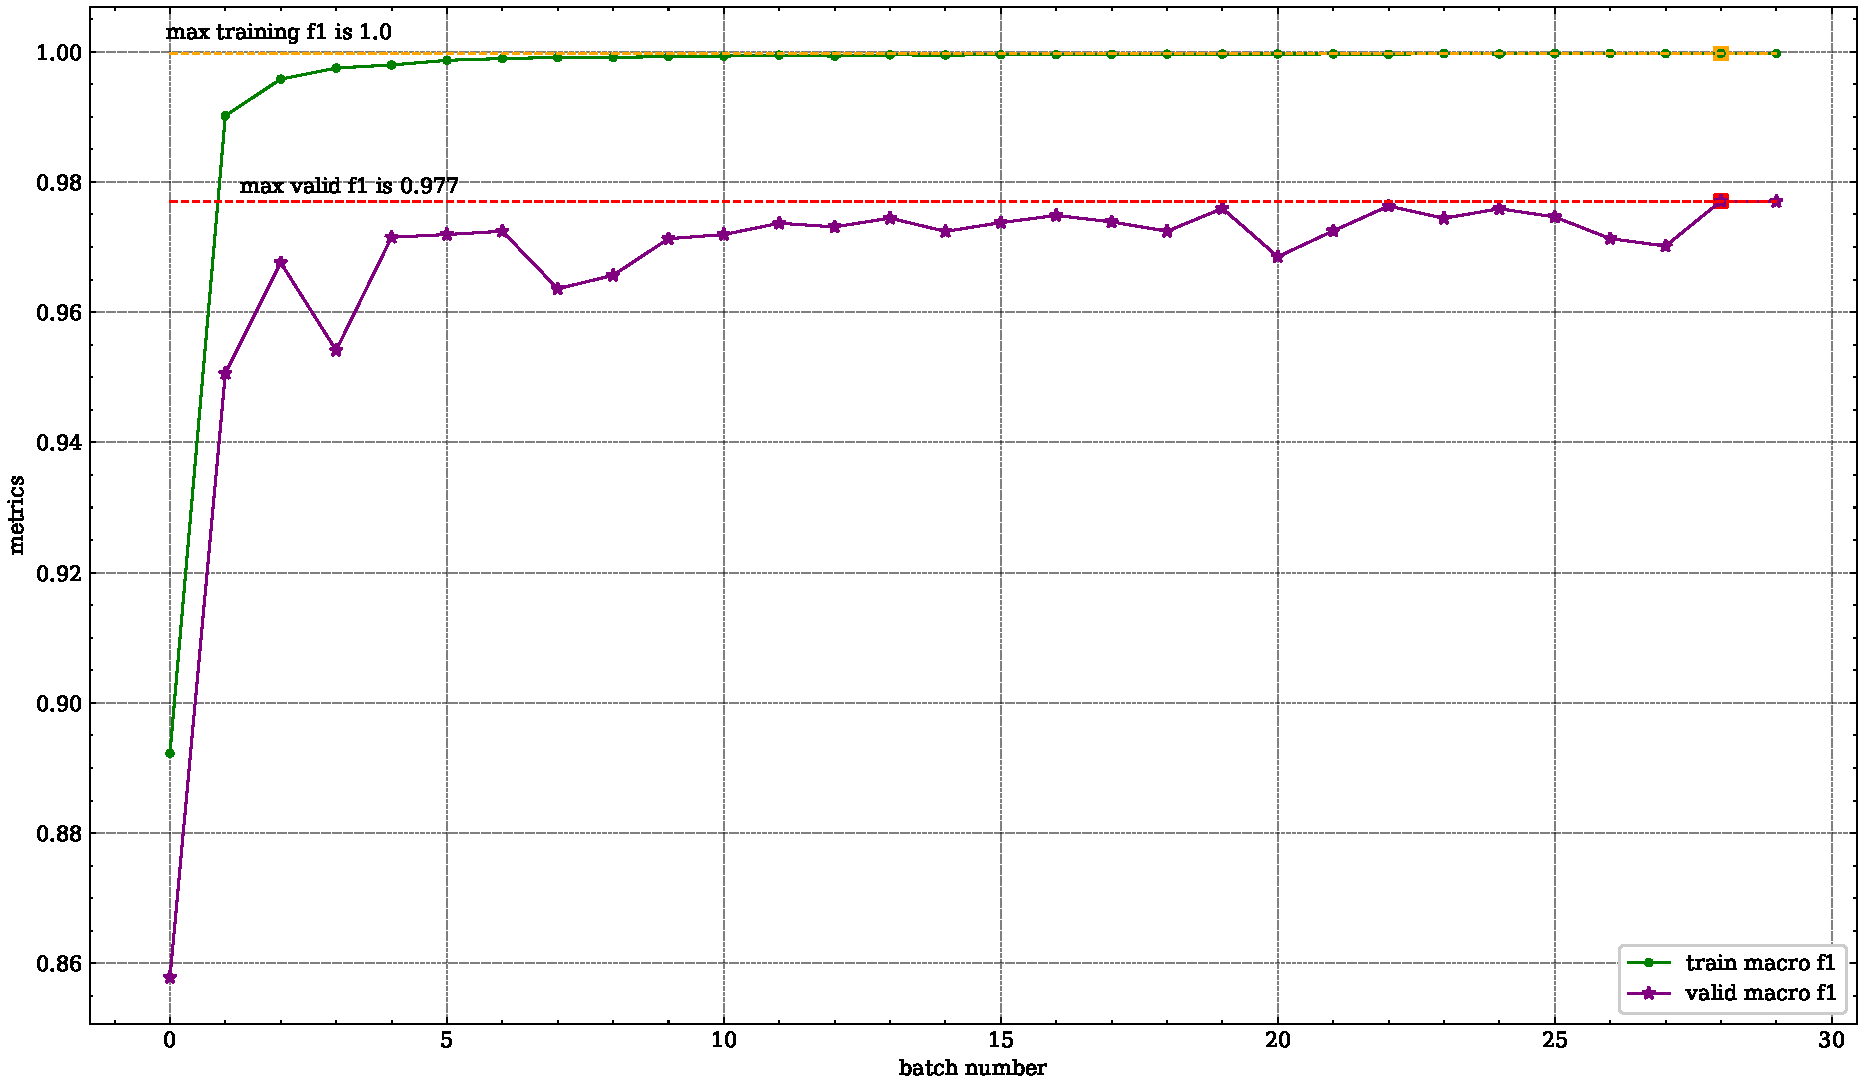
\includegraphics[scale=0.4]{../images/ResNet18训练验证f1.pdf}
		\caption{ResNet18 验证 f1 分数变化图}
		\label{ResNet18训练验证f1}
	\end{center}
\end{figure}

训练完成后,我们分别加载两个模型保存的最优参数进行测试。
在测试中,LeNet\_RB 模型在训练集上的准确率达到了 0.993,f1 分数也达到了 0.993 ;在验证集上的准确率达到了 0.982,f1 分数也达到了 0.952。
ResNet18 模型在训练集上的准确率达到了 1.0,f1 分数也达到了 1.0;在验证集上的准确率达到了 0.992,f1 分数也达到了 0.977。
我们还绘制了两种模型的 ROC 曲线,如图\ref{LeNetRBROC曲线}和\ref{ResNet18ROC曲线}所示。
两种模型的各类别的相关评价指标如表\ref{LeNetRB各类别评价指标}和\ref{ResNet18各类别评价指标}所示。
\begin{figure}[H]
	\begin{center}
		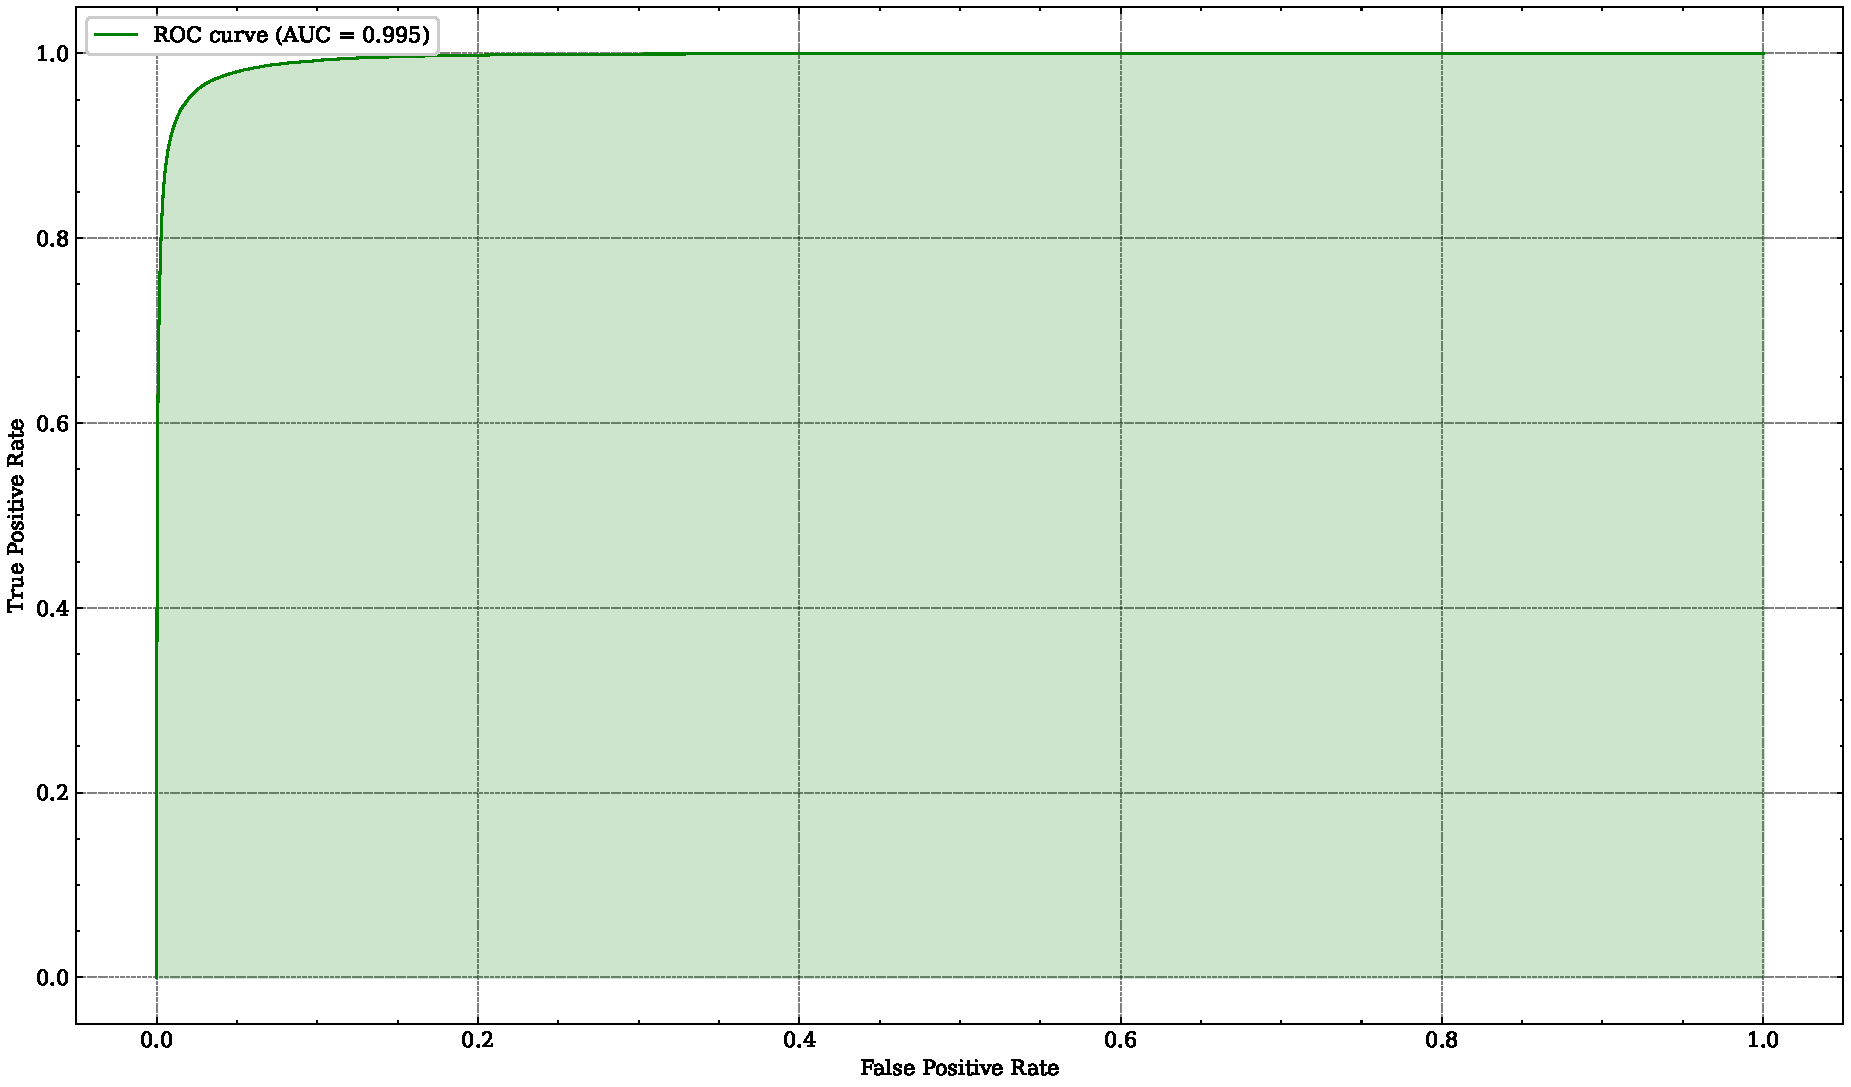
\includegraphics[scale=0.4]{../images/LeNetRBROC曲线.pdf}
		\caption{LeNet\_RB 的 ROC曲线}
		\label{LeNetRBROC曲线}
	\end{center}
\end{figure}
\begin{figure}[H]
	\begin{center}
		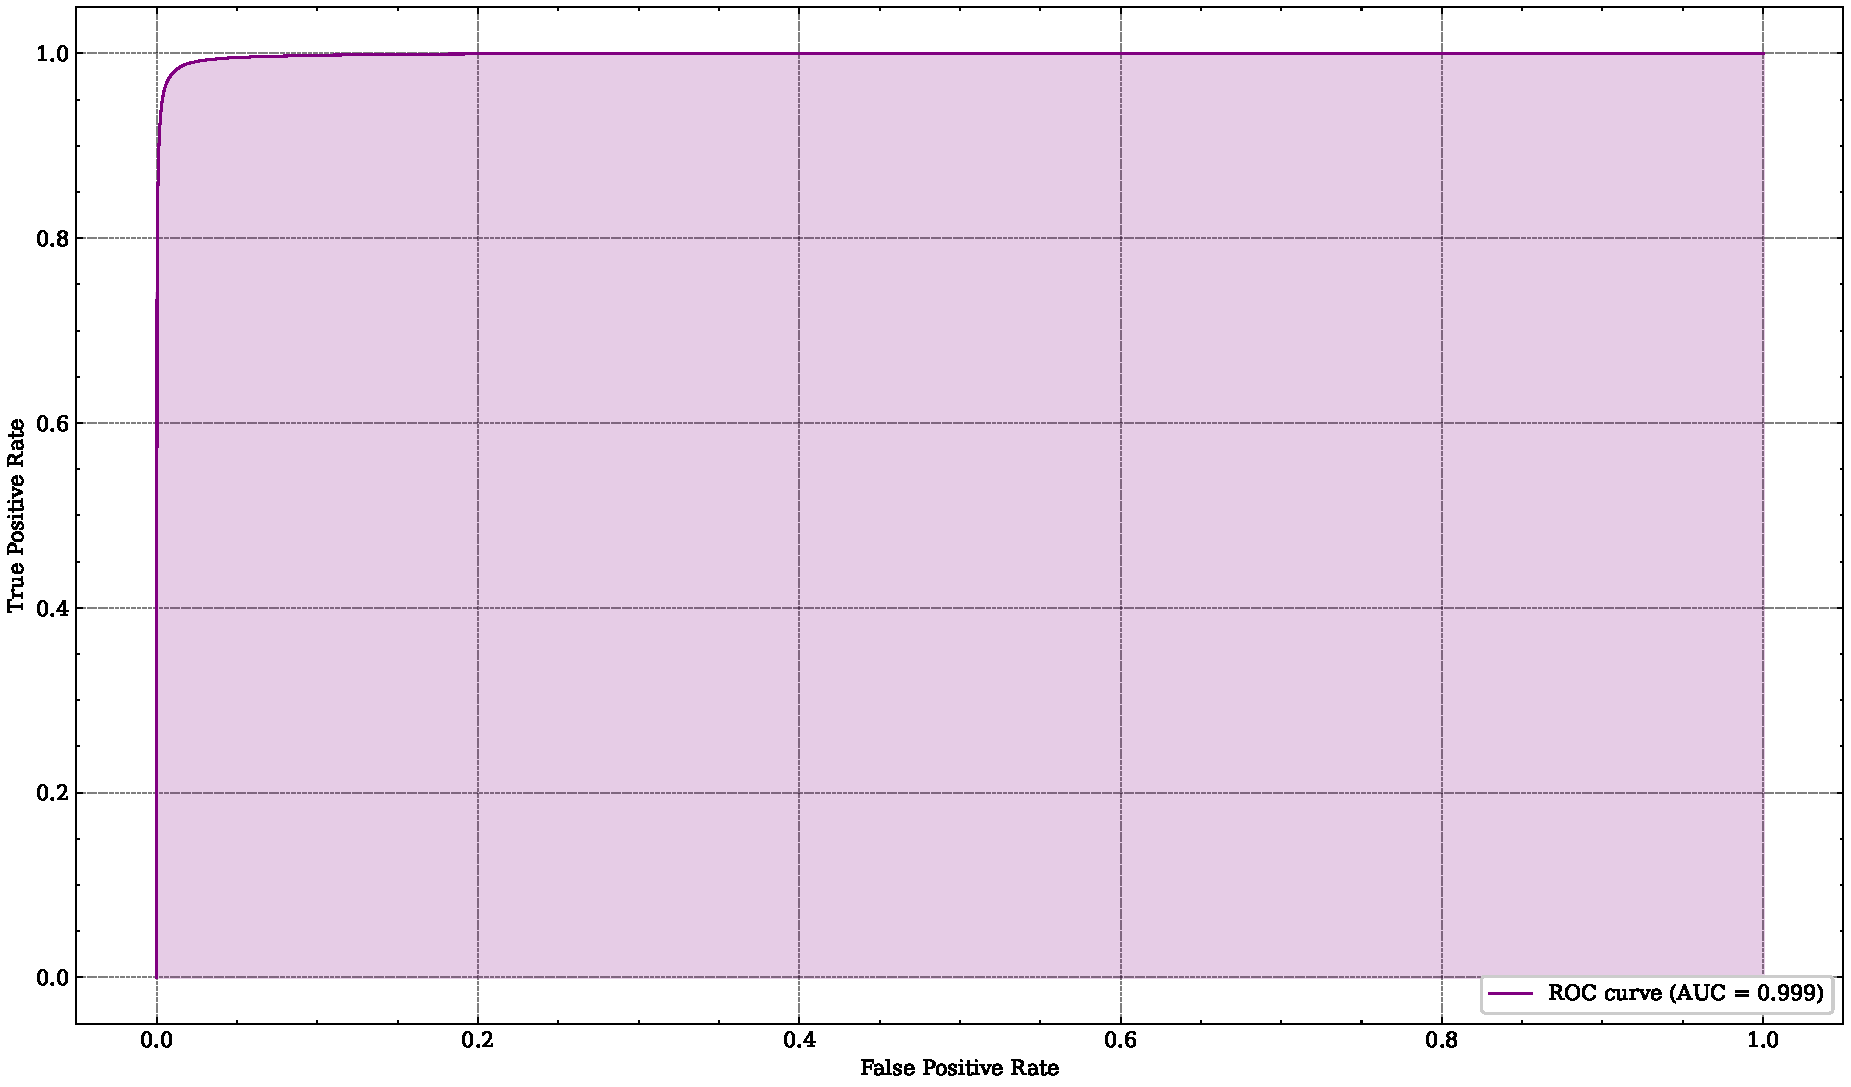
\includegraphics[scale=0.4]{../images/ResNet18ROC曲线.pdf}
		\caption{ResNet18 的 ROC曲线}
		\label{ResNet18ROC曲线}
	\end{center}
\end{figure}

\begin{table}[H]
	\centering
	\caption{LeNet\_RB 各类别的评价指标}
	  \begin{tabular}{ccccc}
		\toprule
			& \textbf{precision} & \textbf{recall} & \textbf{f1-score} & \textbf{support} \\\hline
	  \textbf{0} & 0.99  & 0.98  & 0.99  & 449099 \\
	  \textbf{1} & 0.87  & 0.94     & 0.90  & 51401 \\
	  \textbf{accuracy} &       &       & 0.98  & 500500 \\
	  \textbf{macro avg} & 0.93  & 0.96  & 0.95  & 500500 \\
	  \textbf{weighted avg} & 0.98  & 0.98  & 0.98  & 500500 \\\bottomrule
	  \end{tabular}
	\label{LeNetRB各类别评价指标}
  \end{table}
  \begin{table}[H]
	\centering
	\caption{ResNet18 各类别的评价指标}
	  \begin{tabular}{ccccc}
		\toprule
			& \textbf{precision} & \textbf{recall} & \textbf{f1-score} & \textbf{support} \\\hline
	  \textbf{0} & 0.99  & 1  & 1  & 449099 \\
	  \textbf{1} & 0.97  & 0.95     & 0.96  & 51401 \\
	  \textbf{accuracy} &       &       & 0.99  & 500500 \\
	  \textbf{macro avg} & 0.98  & 0.97  & 0.98  & 500500 \\
	  \textbf{weighted avg} & 0.99  & 0.99  & 0.99  & 500500 \\\bottomrule
	  \end{tabular}
	\label{ResNet18各类别评价指标}
  \end{table}

\section{总结与讨论}
在这一章,我们研究了不同的网络架构对模型准确率的影响。
我们将 LeNet\_RB 和 ResNet18 两种模型的验证评价指标、损失函数变化和 ROC 曲线进行了对比。

首先我们对比模型在验证集上的表现。两种模型在验证集上的最小损失函数值、准确率和 f1 分数如表\ref{模型对比表}所示。
\begin{table}[H]
	\centering
	\caption{模型效果对比表}
	  \begin{tabular}{cccc}
		\toprule
			& \textbf{最小验证损失函数值} & \textbf{准确率} & \textbf{f1 分数} \\\hline
	  \textbf{LeNet\_RB} & 0.062 & 0.982 & 0.952 \\
	  \textbf{ResNet18} & 0.038 & 0.992 & 0.977 \\
	  \bottomrule
	  \end{tabular}
	\label{模型对比表}
  \end{table}

接着,我们对比两者的 ROC 曲线,如图\ref{模型对比ROC曲线}所示。
\begin{figure}[H]
	\begin{center}
		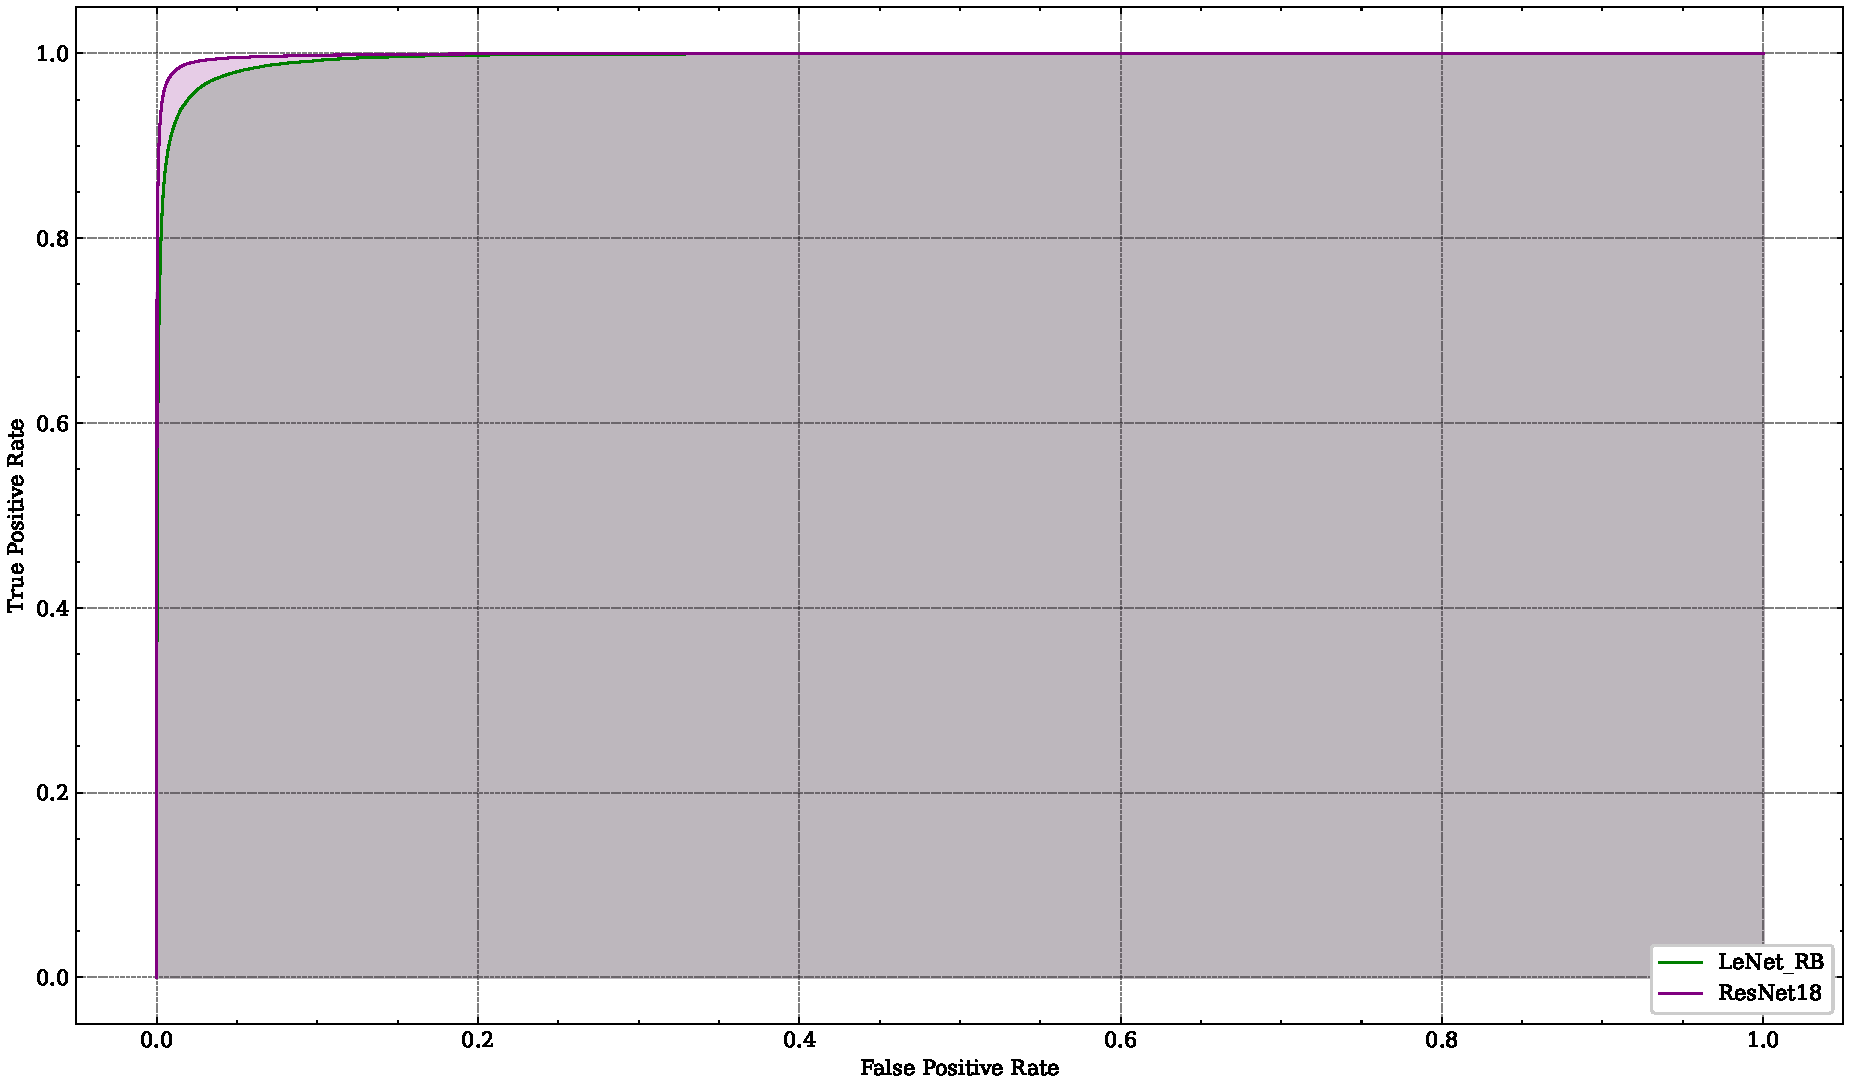
\includegraphics[scale=0.45]{../images/模型对比ROC曲线.pdf}
		\caption{两种模型的 ROC 曲线对比}
		\label{模型对比ROC曲线}
	\end{center}
\end{figure}
  
我们发现,无论是验证集评价指标还是 ROC 曲线,ResNet18 的相关指标均优于 LeNet\_RB。这是由于 ResNet18 的网络层数较多,表达能力较强。
但是 LeNet\_RB 参数较少,其训练和推理用时均明显少于 ResNet18。如果下游任务对实时性要求高,则可以选择 LeNet\_RB;如果对准确性要求高,则可以选择 ResNet18。

\section{实验代码简述}
在本章中,我们简要介绍实验代码的构成。更具体的介绍请见 ReadMe.md 文件。

工作目录中存在 6 个文件和 3 个目录。整个工作目录的结构如下。
\begin{figure}[H]
	\begin{center}
		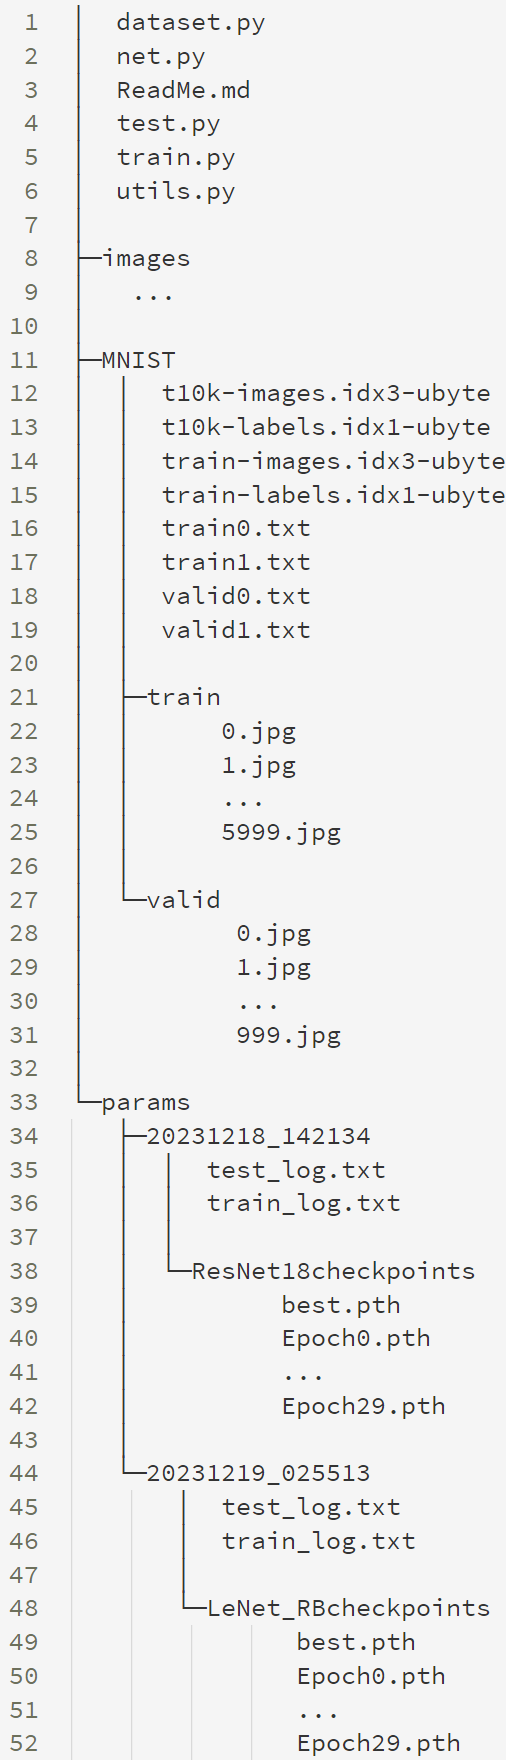
\includegraphics[scale=0.5]{../images/tree.png}
		\caption{工作目录的结构}
	\end{center}
\end{figure}

其中,dataset.csv 是原始数据集。dataset.py 中含有数据预处理的相关函数。net.py 含有模型架构的定义。
ReadMe.md 中介绍了如何对模型进行训练和测试。test.py 是进行模型测试的源代码文件。train.py是进行模型训练的源代码文件。
utils.py 中含有一些工具函数。各函数和类的源代码均含有详细的注释,方便使用者了解其完成的工作。

MNIST 目录存放数据集相关信息。images 目录存放所有绘制的图像。params 目录存放模型的参数。当在源代码中设置存储参数选项为 True 并运行一次 train.py 时,
params 目录中会增加一个以当前时间为名称的子目录。子目录内存放着训练时的日志、每一轮训练结束后的模型参数以及效果最佳的模型参数。当进行模型测试时,测试日志会放置到对应参数所在的子目录中。

\end{document}